\chapter{Differential Forms and Causal Diagrams}
\label{ch-diff-forms}



Commutative diagram
\beq
\xymatrix{
X\ar[r]|f \ar[dr]|\phi
& Y\ar[d]|g
\\
&Z
}
\eeq

Instantiation  of commutative diagram
\beq
\xymatrix{
x\ar[r]|f \ar[dr]|\phi
& y\ar[d]|g
\\
&\Circle{0}
}
\eeq
$\phi(x) = g\circ f (x)$


\section{Review of Differential Forms}

Technically, a
differential form is a $p+1$-form
created by applying the exterior derivative $d$ to a $p$-form,
so a p-form is slightly
more general than a differential
form, but we will seldom
distinguish between the two.
We will mostly use the term p-form
because it is more succinct
and general.



\subsection{Notation}


% Please add the following required packages to your document preamble:
% \usepackage[table,xcdraw]{xcolor}
% Beamer presentation requires \usepackage{colortbl} instead of \usepackage[table,xcdraw]{xcolor}
\begin{table}[]
\begin{tabular}{|l|l|l|}
\hline
 & \cellcolor[HTML]{FFCCC9}Conventional notation & \cellcolor[HTML]{FFCCC9}My notation \\ \hline
\cellcolor[HTML]{9AFF99}pullback & $\phi^*(\cdot)$ & $\phi^{PB}(\cdot)$ \\ \hline
\cellcolor[HTML]{9AFF99}\begin{tabular}[c]{@{}l@{}}vector field\\ .\end{tabular} & $X$ & $\vecX$ \\ \hline
\cellcolor[HTML]{9AFF99}\begin{tabular}[c]{@{}l@{}}coordinate vector\\ .\end{tabular} & $\pder{\;}{x^i}$ & $\vecpder{x^i}$ \\ \hline
\cellcolor[HTML]{9AFF99}\begin{tabular}[c]{@{}l@{}}partial derivative\\ .\end{tabular} & $\pder{\;}{x^i}$ & $\pder{\;}{x^i}$ or  $(\vecpder{x^i})^{op}$ \\ \hline
\cellcolor[HTML]{9AFF99}p-form & $\omega$ (Greek letters) & $\ul{\omega}$ or, more explicitly, $\pform{\omega}{p}$ \\ \hline
\cellcolor[HTML]{9AFF99}metric & $g$ & $\metric$ \\ \hline
\cellcolor[HTML]{9AFF99}group $G$ element & $g$ & $g$ \\ \hline
\cellcolor[HTML]{9AFF99}\begin{tabular}[c]{@{}l@{}}covariant derivative\\ (acts on frame $\vece_\mu$)\end{tabular} & $\nabla_\mu$ & $\nnabla_\mu$ \\ \hline
\cellcolor[HTML]{9AFF99}\begin{tabular}[c]{@{}l@{}}flat space gradient (treats \\ frame $\vece_\mu$ as a constant)\end{tabular} & $\partial_\mu$ & $\partial_\mu=\nabla_\mu$ \\ \hline
\end{tabular}
\caption{Comparison of conventional and my notation for differential geometry}
\label{tab-compare-notation-differ-geo}
\end{table}

\subsection{Preliminaries}
\hrule
 Index bracket notation

antisymmetric part, antisymmetrization
\beq
T_{A(\alp\beta)}=\frac{1}{2}
\underbrace{(T_{\alp\beta}-T_{\beta\alp})}_
{T_{UA(\alp \beta)}}
\eeq
$UA=$ un-normalized antisymmetrization

symmetric part, symmetrization
\beq
T_{S(\alp\beta)}=\frac{1}{2}
\underbrace{(T_{\alp\beta}+T_{\beta\alp})}_
{T_{US(\alp \beta)}}
\eeq
$US=$ un-normalized symmetrization

\beq
T_{\alp \beta}=
T_{A(\alp\beta)}+ T_{S(\alp\beta)}
\eeq

\beq
T_{A(\alp\beta)}= - T_{A(\beta\alp)}
\eeq

\beq
T_{S(\alp\beta)}=  T_{S(\beta\alp)}
\eeq


\beqa
T_{A(\alpha \beta \gamma)}
&=&
\frac{1}{3!}
\underbrace{\sum_{\s \in S_3}
sign(\s)T_{\s(\alpha\beta\gamma)}}_{T_{UA(\alpha \beta \gamma)}}
\\
&=&
\frac{1}{3!}
\left[
T_{\alp\beta\gamma}
+
SP(\alp\beta\gamma)\neq  I
\right]
\eeqa
$SP(\alp\beta\gamma)\neq  I$ means
signed permutations not equal to identity

\beqa
T_{S(\alpha \beta \gamma)}
&=&
\frac{1}{3!}
\underbrace{\sum_{\s \in S_3}
T_{\s(\alpha\beta\gamma)}}_{T_{US(\alpha \beta \gamma)}}
\\
&=&
\frac{1}{3!}
\left[
T_{\alp\beta\gamma}
+
UP(\alp\beta\gamma)\neq  I\right]
\eeqa
$UP(\alp\beta\gamma)\neq  I$ means
unsigned permutations not equal to identity


\beq
T_{\alp\beta\gamma}
=
T_{A(\alp\beta\gamma)}
+
T_{S(\alp\beta\gamma)}
\eeq




\subsection{Tangent Vectors, Vector Fields}

Let

$M=$ \qt{base} manifold (e.g. the surface of a sphere or Mobius strip)

$\pi=$ a
point on $M$

$T_\pi (M)=$
tangent space at $\pi$.
A vector space.

$\ZZ_1^n = \{ 1,2,\ldots n\}$

$n=$ dimension of $T_\pi(M)$.

$\{\vece_i\mid i\in \ZZ_1^n\}=$ {\bf tangent basis (t-basis)}, a basis for $T_\pi(M)$. These vectors need not be orthogonal nor normalized.

$\{\check{x}_i\mid i\in \ZZ_1^n\}=$ {\bf coordinate t-basis}
for coordinates
$\{x^i\}_{i=1}^n$ , a special t-basis for $T_\pi(M)$.
Unlike the generic t-basis
$\{\vece_i\}_{i=1}^n$, a coordinate t-basis
is guaranteed to come from a coordinate system $\{x^i\}_{i=1}^n$ on $M$
for which differentiable functions $f(x^1, x^2, \cdots, x^n)$ exist.
 As with the basis  $\{\vece_i\}_{i=0}^n$, the  t-basis $\{\vecpder{x^i}\}_{i=0}^n$ need not be orthogonal nor normalized.

A {\bf tangent vector} $\vec{v}\in T_\pi(M)$
lives at a single point $\pi\in M$.
A {\bf tangent vector field} $\vecX:
M\rarrow \cup_{\pi\in}T_\pi(M)$ assigns a vector $X(\pi)$
 to every point $\pi\in M$.
\footnote{
A p-form $\ul{\omega}$ (defined later) is also defined pointwise. When we write
$\ul{\omega}(\vecX, \vecY)$,
we really mean the function
$\pi \mapsto
\ul{\omega}(\vecX(\pi), \vecY(\pi))
$}

The set\footnote{$\sqcup$ is the symbol for the disjoint union, i.e., the union minus all the overlaps.} $T(M)=\sqcup_{\pi\in M}T_\pi(M)$
is called the {\bf fibre bundle}
of $M$. Each
$T_\pi(M)$ is a fibre.
$T(M)$ has dimension $2n$.

Let
\beq
\vec{r}= x^i\vecpder{x^i},
\quad d\vecr = dx^i \vecpder{x^i}
\eeq
Then
\beq
\vecpder{x^i}=
\frac{\partial\vec{r}}{\partial x^i},\quad
(\vecpder{x^i})_{op}=
\pder{\;}{x^i}\quad\text{(op=operator)}
\eeq
\beq
\hat{x}_i = \frac{\vecpder{x^i}}{|\vecpder{x^i}|}
\eeq

If
\beq
\vecV=V^i \vecpder{x^i},
\eeq
then

\beq
\vecV_{op}=\vecV\cdot \nabla=
 V^i\frac{\partial}{\partial x^i},
\quad \vecV_{op} \vec{r}
=\vecV
\eeq


\ul{It's conventional
to use} $\pder{\;}{x^i}$
\ul{to denote both
$\vecpder{x^i}$ and
$(\vecpder{x^i})_{op}$,
but we won't follow
that convention here.}


Early workers in this field
refer to
a coordinate t-basis as a {\b holonomic} t-basis.
The word \qt{holonomic}
comes from the Greek
words \qt{holos}=whole or complete
and \qt{nomos}=a rule
or prescription.

In Mechanics, a {\bf holonomic (or integrable) constraint}
is one that can be
written exclusively
in terms of the coordinates of the system and time:

\beq
f(\vecr, t)=0
\eeq
where $\vecr=(x^1, x^2, \dots, x^n)$.
By contrast, a {\bf non-holonomic (or non-integrable)
constraint} involves velocities:

\beq
g(\vecr, \dot{\vecr}, t)=0
\eeq

In differential geometry, the term holonomic refers to a t-basis of vectors
$\{\vece_i\}_{i=0}^n$
for which there exists
a coordinate system
$\{x^i\}_{i=1}^n$
and a vector field\\
$\vecr(x^1, x^2, \cdots, x^n)$ such that

\beq
\vece_i = \pder{\vecr}{x^i}
\eeq
for all $i\in\ZZ_1^n$.
In conclusion,
a coordinate t-basis and
a holonomic t-basis are
the same thing.

A t-basis $\{\vece_i\}_{i=1}^n$ is a coordinate=holonomic
t-basis iff
\beq
[(\vece_i)_{op},
(\vece_j)_{op}]=0
\eeq
for all $i,j\in\ZZ_1^n$.
For example, for Cartesian coordinates
in 2-dim,
\beq
d\vecr = dx \hat{x} + dy  \hat{y}
\eeq
so
$(\hat{x}, \hat{y})$
is holonomic because

\beq
\ul{d\vecr} = \ul{dx} \hat{x} + \ul{dy}  \hat{y}
=
\ul{dx} \pder{\vecr}{x}
+ \ul{dy} \pder{\vecr}{y}
\eeq

\beq
 \left[\pder{\vecr}{x}\right]_{op}=
\pder{\;}{x},\quad
\left[\pder{\vecr}{y}\right]_{op}
=\pder{\;}{y}
\eeq



\beq
\left[\pder{\;}{x}, \pder{\;}{y}
\right]=0
\eeq
For polar coordinates in 2-dim,

\beq
d\vecr =
dr \hat{r} + rd\theta \hat{\theta}
\eeq

$(\hat{r}, \hat{\theta})$ is a non-holonomic t-basis because

\beq
\ul{d\vecr} =
\ul{dr} \hat{r} + \ul{rd\theta} \hat{\theta}=
\ul{dr} \pder{\vecr}{r}
+
\ul{rd\theta}
\left[\frac{1}{r}\pder{\vecr}{\theta}
\right]
\eeq

\beq
 \left[\pder{\vecr}{r}\right]_{op}=
\pder{\;}{r},
\quad
\left[
\frac{1}{r}\pder{\vecr}{\theta}\right]_{op}
=\frac{1}{r}\pder{\;}{\theta}
\eeq

\beq
\left[
\pder{\;}{r},
\frac{1}{r}\pder{\;}{\theta}
\right]\neq 0
\eeq
On the other hand,
$(\hat{r}, r\hat{\theta})$
is a holonomic t-basis because

\beq
\ul{d\vecr} =
\ul{dr} \hat{r} + \ul{d\theta} r\hat{\theta}=
\ul{dr} \pder{\vecr}{r}
+
\ul{d\theta} \pder{\vecr}{\theta}
\eeq

\beq
 \left[\pder{\vecr}{r}\right]_{op}=
\pder{\;}{r},
\quad
\left[\pder{\vecr}{\theta}\right]_{op}
=\pder{\;}{\theta}
\eeq

\beq
\left[
\pder{\;}{r},
\pder{\;}{\theta}
\right]= 0
\eeq

In the General Relativity section \ref{sec-gen-rel},
we will introduce
the so called tetrad
(vierbein) t-basis. That t-basis is non-holonomic too.

A t-basis 
$\{\vece_i\}_{i=1}^n$ is orthogonal if
$(\vece_i)^a 
(\vece_j)_a=0$ for all $i\neq j$. That t-basis is saidd to be normalized if $(\vece_i)^a 
(\vece_i)_a= 1$
for all $i$.
A basis is orthonormal if it is
both  orthogonal
and normalized.
Whether a t-basis
is orthogonal  or normalized has nothing to
do with whether it is holonomic or not.

\begin{table}[h!]
\begin{tabular}{|l|l|l|}
\hline
\begin{tabular}[c]{@{}l@{}}My notation for\\ t-basis vectors\end{tabular} & \cellcolor[HTML]{FFCCC9}not orthonormal & \cellcolor[HTML]{FFCCC9}orthonormal \\ \hline
\cellcolor[HTML]{9AFF99}\begin{tabular}[c]{@{}l@{}}coordinate\\ (holonomic) t-basis\end{tabular} & $\vecpder{x^i}$ & $\hat{x}_i$, e.g., $(\hat{x}, \hat{y})$ \\ \hline
\cellcolor[HTML]{9AFF99}non-holonomic t-basis & $\vece_i$ & $\hate_i$, 
e.g., $(\hat{r}, \hat{\theta})$\\ \hline
\end{tabular}
\caption{My notation for t-basis vectors with various properties. }
\label{tab-basis-notation}
\end{table}




\begin{table}[h!]
\begin{tabular}{|l|l|l|l|l|}
\hline
\rowcolor[HTML]{FFFC9E}
\cellcolor[HTML]{FFFFFF} &  t-basis & dual t-basis & \begin{tabular}[c]{@{}l@{}}displacement \\ vector\end{tabular} &  \\ \hline
\cellcolor[HTML]{DAE8FC}coordinate t-basis & $\vecpder{x^a}$ & $\pform{dx^a}{}$ & $\pform{d\vecr}{}= \vecpder{x^a}\pform{dx^a}{}$ & $\ul{dx^a}(\vecpder{x^b})=\delta^a_b$ \\ \hline
\cellcolor[HTML]{DAE8FC}non-holonomic t-basis & $\vece_a$ & $\pform{\theta^a}{}$ & $\pform{d\vecr}{}=\vece_a\pform{\theta^a}{}$ & $\ul{\theta^a}(\vece_b)=\delta^a_b$ \\ \hline
\end{tabular}
\caption{Notation for coordinate (holonomic) and non-holonomic t-basis.}
\label{tab-basis-dual-basis}
\end{table}





\subsection{p-forms}

When discussing most
concepts about
p-forms, I find it pedagogically
advantageous to define the
concept
first for 0-forms, 1forms, 2-forms
and then
finally the general case of p-forms
(form with $p$ slots).
I will
follow that
strategy in this chapter.


We will always
underline p-forms
and, except in special
cases, use
lower case
Greek letter to represent them.
Sometimes,
we will be even
more explicit and
write
$\pform{\omega}
{p}$ for a
p-form.
$\$^p$, where
represents $p$
place holders or empty slots.



\begin{itemize}
\item  0-form:

\beq
\ul{\omega} = f,\quad
f: M\rarrow \RR
,\quad
\pi \mapsto  f(\pi)
\eeq
For example,
if
\beq
f(x,y)=x^2 + y \quad \text{and}
\quad \pi= (2,3)\eeq
then

\beq f(\pi)= 2^2 + 3= 7
\eeq

\item 1-form:

A 1-form
$\ul{\omega}\in \wedge(M)$ is a LINEAR map

\beq
\ul{\omega}: T_\pi(M)\rarrow \RR,\quad
\vecX\mapsto \ul{\omega}(\vecX)
\eeq
where $\vecX$ is an $n$-dim vector.
$\wedge(M)$ is called the {\bf dual space of $T_\pi(M)$}.

\beq
\ul{\omega}(\vecX)=\sum_{i=1}^n \omega_i \ul{dx^i}(\vecX)
\eeq

$\{\pform{dx^i}{}\mid i\in \ZZ_1^n \}$
are a basis for the 1-forms on $\wedge_\pi(M)$.
They are called the {\bf coordinate dual t-basis} \footnote{
A t-basis is often called a {\bf frame} and a dual t-basis is called a {\bf coframe}. We won't use that nomenclature.} for coordinates
$\{x^i\}_{i=1}^n$.
 They satisfy

\beq
\ul{dx^i}(\vecpder{x^i})=\delta_i^j
\eeq
for $i, j\in\ZZ_1^n$.

For example,
if $\ul{\omega}$ is the following 1-form \pformIN{=2}:
\beq
\pform{\omega}{}= 2 \pform{dx}{}
+ 5 \pform{dy}{},
\quad
\vecX = a \vecpder{x}
+ b \vecpder{y}
\eeq
then,
using $\ul{dx^i}(\vecpder{x^j})=\delta(i,j)$,

\beq
\ul{\omega}(\vecX)=
2a + 5b
\eeq

\item 2-form:

A 2-form
$\ul{\omega}\in \wedge_\pi(M)\wedge \wedge_\pi(M)=\wedge^2_\pi(M)$
is a LINEAR map
\beq
\ul{\omega}: T_\pi(M)\times T_\pi(M)=T^2_\pi(M)\rarrow \RR,\quad (\vecX,\vecY)\mapsto \ul{\omega}(\vecX, \vecY)
\eeq
where $\vecX$ and $\vecY$ are n-dim vectors.

\beq
\ul{\omega}(\vecX, \vecY)=\sum_{1\leq i < j\leq n} \omega_{ij} \ul{dx^i}(\vecX)
\wedge \ul{dx^j}(\vecY)
\eeq

\beq
\pform{dx^i}{}\wedge \pform{dx^j}{}=\pform{dx^i \wedge dx^j}{2}
\eeq

\beq
\ul{dx^1}\wedge \ul{dx^1}=
\ul{dx^2}\wedge \ul{dx^2}=0
\eeq

\beq
\ul{dx^1}\wedge \ul{dx^2}=
-\ul{dx^2}\wedge \ul{dx^1}
\eeq


$\{\pform{dx^i}{}
\wedge \pform{dx^j}{}\mid
i\in \ZZ_1^n, j\in \ZZ_1^n,
i<j\}$
are a basis for the 2-forms on $T_\pi(M)\times
T_\pi(M)$. They satisfy

\beq
\ul{dx^i}(\vecX)
\wedge \ul{dx^j}(\vecY)=
\ul{dx^i}(\vecX)
\otimes \ul{dx^j}(\vecY)
-
\ul{dx^i}(\vecY)
\otimes \ul{dx^j}(\vecX)
\eeq
for $i, j\in\ZZ_1^n$.
Hence,

\beq
\ul{dx^1}(\vecX)\wedge\ul{dx^2}(\vecY)=
-\ul{dx^1}(\vecY)\wedge\ul{dx^2}(\vecX)
\eeq
In other words, these basis elements
 change sign
if you exchange the
arguments $\vecX$ and $\vecY$.



For example, if
$\ul{\omega}$ is
the following 2-form \pformIN{=2}

\beq
n=2,\quad
\ul{\omega}=
\ul{dx}\wedge \ul{dy},\quad
\vecX= X^1 \vecpder{x}
+ X^2 \vecpder{y}
,\quad
\vecY= Y^1 \vecpder{x}
+ Y^2 \vecpder{y}
\eeq
then
\beq
\ul{\omega}(\vecX,\vecY)= X^1 Y^2 -
X^2 Y^1= X^{UA(1}Y^{2)}
\eeq

\item p-forms

A p-form $\ul{\omega}\in
\underbrace{\wedge_\pi(M)\wedge \cdots \wedge \wedge_\pi(M)}_{\text{$p$ copies of $\wedge_\pi(M)$}}=
\wedge^p_\pi(M)$ is a LINEAR map

\beq
\begin{array}{l}
\ul{\omega}:
\underbrace {T_\pi(M)
\times
\cdots
T_\pi(M)}_{
\text{ $p$ copies of } T_\pi(M)}=T^p_\pi(M)
\rarrow \RR,
\\
(\vecX^{(1)}, \vecX^{(2)}, \ldots, \vecX^{(m)})\mapsto
\ul{\omega_\pi}(\vecX^{(1)}, \vecX^{(2)}, \ldots, \vecX^{(m)})
\end{array}
\eeq
where $\vecX^{(j)}$ for $j=1, 2, \dots p$ are n-dim vectors.

Let

\beq
\ul{\otimes  dx^{i_1 i_2\cdots i_p}}
(\vecX^{(1)}, \vecX^{(2)}, \ldots, \vecX^{(p)})
=
\ul{dx^{i_1}}(\vecX^{(1)})
\otimes
\ul{dx^{i_2}}(\vecX^{(2)})
\otimes \cdots
\otimes
\ul{dx^{i_p}}(\vecX^{(p)})
\eeq
where $\otimes $ is
Cartesian (order preserving) product for reals.

\beq
\ul{\wedge dx^{i_1 i_2\cdots i_p}}
(\vecX^{(1)}, \vecX^{(2)}, \ldots, \vecX^{(p)})
=
\ul{dx^{i_1}}(\vecX^{(1)})
\wedge
\ul{dx^{i_2}}(\vecX^{(2)})
\wedge\cdots
\wedge
\ul{dx^{i_p}}(\vecX^{(p)})
\eeq



\beq
\cali^p =\{ I\mid I=(i_1, i_2, \cdots, i_p) , \quad 1\leq i_1, i_2,\cdots ,i_p\leq n\}
\eeq

\beq
\cali^p_< =\{ I\mid I=(i_1, i_2, \cdots, i_p) , \quad 0\leq i_1< i_2<\cdots <i_p\leq n\}
\eeq

\beq
\pform{\omega}{p}=
\sum_{I \in \cali^p_<} \omega_I
\pform{\wedge d x^I}{p}
=
\frac{1}{p!}
\sum_{I \in \cali^p}
\omega_I \pform{\wedge d x^I}{p}
\eeq


$\{\pform{\wedge dx^I}{}
\mid I\in
\cali^p_<\}$
are a basis for the p-forms on $T^p_\pi(M)$. They satisfy

\beq
\ul{\wedge dx^I}(\vecX^{(I)})=
\sum_{\s\in S_p}sign(\s)
\ul{\otimes dx^I}(\vecX^{(\s(I))})
=
\ul{\otimes dx^I}(\vecX^{UA(I)})
\eeq
for $I \in \cali^p$,
where $\s$ ranges over all possible permutations of $p$ symbols.
Hence,

\beq
\ul{\wedge dx^I}(\vecX^{(I)})=
-\ul{\wedge dx^I}(\vecX^{(\s (I))})
\eeq
if $\s$ is a swap (transposition)
of any two symbols of $I$.
In other words, these basis elements
 change sign
if you exchange any two
arguments $\vecX$ and $\vecY$.


\end{itemize}

\subsection{Metric}




Given two vector fields
$\vecU = U^i \vecpder{x^i}$,
and $\vecV = V^i \vecpder{x^i}$,
the metric function $\metric(\vecU, \vecV)$ satisfies
\beq
\metric(\vecU, \vecV)=
\metric(\vecV, \vecU) = V^i U^j
\underbrace{\metric(\vecpder{x^i}, \vecpder{x^j})}_{\vecpder{x^i}
\cdot\vecpder{x^j}=\metric_{ij}}
\eeq

Let $\metric$ represent the metric
matrix
\beq
\metric = [\metric_{ij}]=
\left[
\ul{\metric}(\vece_i, \vece_j)
\right]
\eeq

The old fashioned way of 
presenting a metric is as a
quadratic form of 
differentials:

\beq
|d\vecr|^2 = (ds)^2 =
\metric_{ij}dx^i \; dx^j
\eeq
For example, in 
polar coordinates $(r, \theta)$,
we have
$\metric=diag(1, r^2)$ so
$(ds)^2 = (dr)^2 + r^2 (d\theta)^2$.

\begin{itemize}

\item signature

The {\bf signature} of metric $\metric$
is $(N^-, N^+)$, where $N^+$ (resp., $N^-$)
is  number of positive (resp., negative) eigenvalues. A metric 
with $N^-=0$ is  said to be 
a {\bf \Rien metric}.

\item $\metric$ is symmetric

\beq
\metric^T  =\metric
\eeq

\beq
\metric_{ij}=\metric_{ji}
\eeq
\item inverse of $\metric$

\beq
\metric^{-1}=[\metric^{ij}]=
[\ul{\metric^{-1}}(\ul{\theta}^i, \ul{\theta}^j)]
\eeq

\beq
\metric_{ij}\metric^{jk}= \delta_i^k
\eeq

Note that this does not imply $\metric=\metric^{-1}$.
In general, $\metric$ and $\metric^{-1}$ are different.
For example, in polar 
coordinates, $\metric=diag(1, r^2)$, $\metric^{-1}= (1, 1/r^2)$.

\item raising and lowering indices with $\metric$
\beq
V_j = V^i \metric_{ij},\quad
V^j = V_i\metric^{ij}
\eeq

\item computing magnitude of a vector with $g$
\beq
|\vecV|^2 = \metric(\vecV, \vecV)=
V^i V^j \metric_{ij}= V^i V_i
\eeq
\item inner product
\beqa
\av{\vecpder{x^i}, \vecpder{x^j}}&=& \metric_{ij}
\\
\av{\ul{dx^i},\vecpder{x^j}} &=&
\ul{d x^i} (\vecpder{x^j})=\delta_i^j
\\
\av{\ul{dx^i}, \ul{dx^j}}&=&
\metric^{ij}
\eeqa




\beq
\left\{
\begin{array}{l}
\pform{\alp}{}=
\alp_i\pform{dx^i},
\quad
\pform{\beta}{}=
\beta_i\pform{dx^i}{}
\\
\vecU = U^i \vecpder{x^i},
\quad
\vecV = V^i \vecpder{x^i}
\end{array}
\right.
\eeq

\beqa
\metric(\vecU,\vecV)&=&
\av{\vecU,\vecV}=
U^i V^j
\underbrace{\metric(\vecpder{x^i}, \vecpder{x^j})}_{\metric_{ij}}
\\
\metric(\ul{\alp},\vecV)&=&
\av{\ul{\alp},\vecV}=
\alp_i V^j
\underbrace{\metric(\ul{dx}^i, \vecpder{x^j})}_{\delta^i_j}
\\
\metric(\ul{\alp},\ul{\beta}) &=&
\av{\ul{\alp},\ul{\beta}}=
\alp_i \beta_j
\underbrace{\metric(\ul{dx}^i,\ul {dx^j}
)}_{\metric^{ij}}
\eeqa

p-forms

\beq
\pform{\alp}{p}=\sum_{I\in \cali^p_<}\alp_I \pform{\wedge dx^I}{p},
\quad
\pform{\beta}{q}=\sum_{I\in \cali^q_<}\beta_I \pform{\wedge dx^I}{q}
\eeq

\beq
\av{\pform{\alp}{p}, \pform{\beta}{q} }=
\left\{
\begin{array}{ll}
0& \text{if $p\neq q$}
\\
\sum_{I\in \cali^p_<}
\alp_I \beta_I
&\text{if $p=q$}
\end{array}
\right.
\label{eq-point-inner-p}
\eeq
The inner product of p-forms
Eq.(\ref{eq-point-inner-p})
is point-wise. It's also possible
to define a global inner 
product of p-forms by
integrating the pointwise
inner product over the manifold $M$

\beq
\av{\pform{\alp}{p}, \pform{\beta}{p}}_M=
\int_M dV\;
\av{\pform{\alp}{p}, \pform{\beta}{p}}
\label{eq-global-inner-p}
\eeq

\end{itemize}

Examples
\begin{enumerate}
\item Polar coordinates $(r, \theta)
\in \RR\times [0, 2\pi]$



\beq
|\vecpder{r}|^2 = \metric(\vecpder{r}, \vecpder{r})=1,
\quad
|\vecpder{\theta}|^2=
\metric(\vecpder{\theta}, \vecpder{\theta})=r^2,\quad
\metric(\vecpder{r}, \vecpder{\theta})=0
\eeq

\beq
\metric=[\metric_{ij}] = diag(1, r^2)
\eeq
If $dx^i=[dr, d\theta]$ then

\beq
\metric_{ij}dx^i dx^j= (dr)^2 + r^2 (d\theta)^2
\eeq


\item Euclidean 3-dim space, $(x,y,z)\in \RR^3$

\beq
\metric(\vecpder{x^i}, \vecpder{x^j}) = diag(1, 1, 1)
\eeq

\item Spacetime,
$(t, x, y, z)\in\RR^4$

\beq
\metric(\vecpder{x^i}, \vecpder{x^j}) = diag(-1, 1, 1, 1)
\eeq
(or $-diag(-1, 1, 1, 1)$ in some textbooks)

\item

\beq
S\indices{^{ij}_{rst}}=
S(\ul{dx^i}, \ul{dx^j}, \vecpder{x^r}, \vecpder{x^s}, \vecpder{x^t})
\eeq
\end{enumerate}



\subsection{Pullback map}

Suppose functions
$\phi: X\rarrow Y$ and $f: Y\rarrow Z$  satisfy

\beq
\xymatrix{
X\ar[r]|\phi
\ar[dr]|{f\circ \phi}
&Y\ar[d]|f
\\
& Z
}
\eeq
The {\bf pullback function} $\phi^{PB}$
\footnote{$\phi^{PB}$
is often denoted by $\phi^*$.}
maps the function $f$
to the function $f\circ\phi$.

\beq
\xymatrix@C=5pc{
x\ar[r]|\phi
\ar[rd]|{\phi^{PB}}
& \phi(x)(=y)\ar[d]|f
\\
& \phi^{PB}(f)(x)(=f\circ\phi(x))
}
\eeq

\beq
\phi^{PB}(f) (x)= f(\underbrace{\phi(x)}_y)=
f\circ \phi(x)
\eeq

\beq
\phi^{PB}(f) = f\circ\phi
\eeq

The  pullback function
is seldom used by physicists.
They will either use $f(\phi(x))$ only,
or they will
write slightly confusing statements like
$f(x)= f(y)$ (as they do in Thermodynamics, were they
write statements like $U(S, V)= U(P, T)$
instead of $U(S, V)= U(\phi(P, T))$.\quad).
It's a tradeoff. Not using pullback functions makes
the notation
more succinct but less precise. Using the pullback
function can make some
statements more symmetrical too. (for example, $\phi(U)(P, T)$ looks better than $U(\phi(P, T))$.\quad).



\subsection{Exterior Derivative}


\beq
d\;\pform{\omega}{p}=
\pform{d\omega}{p+1}
\eeq

\begin{itemize}
\item $d$ acting on 0-form $f(x)$:
\beq
\pform{df}{}= \sum_i \pder{f}{x^i}\pform{dx^i}{}
\eeq

\item $d$ acting on 1-form $\pform{\omega}{}$:

\beq
\pform{\omega}{}= \sum_{i=1}^n \omega^i\pform{dx^i}{}
\eeq



\beqa
\pform{d\omega}{2} &=&
\sum_{i,j}
\pder{\omega^i}{x^j}
\pform{dx^j}{}
\wedge\pform{dx^i}{}
\\
&=&
\sum_{(i,j)\ni i<j}
\left[
\pder{\omega^i}{x^j}
-
\pder{\omega^j}{x^i}
\right]
\pform{dx^j}{}
\wedge\pform{dx^i}{}
\eeqa

\beq
a_{12}\;
\ul{dx^1}\wedge \ul{dx^2}
 +
a_{21}\;
\ul{dx^2}\wedge \ul{dx^1}
=
(a_{12}-a_{21})
\ul{dx^1}\wedge \ul{dx^2}
\eeq


\item $d$ acting on p-form $\pform{\omega}{p}$:

\beq
\pform{\omega}{p}=
\frac{1}{p!} \sum_{I\in \cali^p} \omega^I\pform{\wedge dx^I}{p}
\eeq



\beqa
\pform{d\omega}{p+1} &=&
\frac{1}{p!}
\sum_{j=1}^n \sum_{I\in \cali^p}
\pder{\omega^I}{x^j}
\pform{dx^j}{}
\wedge\pform{\wedge dx^I}{p}
\\
&=&
\frac{1}{p!}
\sum_{(j,I)\in \cali^{p+1}}
\pder{\omega^I}{x^j}
\pform{\wedge dx^{j, I}}{p+1}
\\
&=&
\underbrace{\frac{(p+1)!}{p!}}_{p+1}
\sum_{(j,I)\in \cali^{p+1}_<}
\pder{\omega^I}{x^j}
\pform{\wedge dx^{j, I}}{p+1}
\eeqa

For $p=1$, this reduces to

\beqa
\pform{d\omega}{2} &=&
2  \sum_{(j, i) \in \cali^2_<}
\pder{\omega^i}{x^j}
\pform{dx^j}{}\wedge
\pform{dx^i}{}
\\
&=&
\sum_{(j, i) \in \cali^2_<}
\left[\pder{\omega^i}{x^j}
-
\pder{\omega^j}{x^i}
\right]
\pform{dx^j}{}\wedge
\pform{dx^i}{}
\eeqa
as expected.

\end{itemize}


\begin{claim}
For any two p-forms
$\pform{\alp}{p}$
and $\pform{\beta}{q}$
and function $f(x)$

\beq
d(f\ul{\alp})=
\ul{df}\wedge \ul{\alp}
\eeq

\beq
d(\ul{\alp} + \ul{\beta})=
d\ul{\alp} + d\ul{\beta}
\eeq

\beq
d(\ul{\alp}\wedge \ul{\beta})=
d\ul{\alp}\wedge \ul{\beta}
+(-1)^{pq}
\ul{\alp}\wedge d\ul{\beta}
\eeq

\beq
d(d\ul{\alp})=0
\eeq
\end{claim}
\proof
\qed

\hrule Exact and Closed 1-form

\beq
\begin{array}{ccc}
\xymatrix{
f(\cdot)\ar[d]|d
\\
\pform{\omega}{}
}
&&
\xymatrix{
\pform{\omega}{}
\ar[d]^d
\\
\Circle{0}
}\\
\text{$\pform{\omega}{}$ Exact 
(\qt{from-$d$}})
&& \text{$\pform{\omega}{}$  Closed (\qt{no-$d$}})
\\
\exists \text{ \qt{potential function}} f(x) \ni \pform{\omega}{}=\pform{df}{}
&&
d\pform{\omega}{}=0
\end{array}
\eeq

Clearly, $\pform{\omega}{}\text { exact} \implies \pform{\omega}{} \text{ closed}$.
The converse is true locally
but not globally.
For example, consider the 1-form $\ul{d\theta}$ for polar coordinates 
$(r, \theta)$
with $M=$ the puncture plane $\RR^2-\{(0,0)\}$. $d(\ul{d\theta})=0$ so $\ul{d\theta}$ is closed but 
$\int_0^{2\pi} d\theta =2\pi$ so there is no continuous 
function $\alp$, (unlike $d\theta$ which is not continuous because it jumps at the cut)  defined over all $M$ such that $d\theta = d\alp$. Otherwise,
$\int_{0}^{2\pi} d\theta= \int_{0}^{2\pi} d\alp = 0$.


\subsection{Hodge star operator}

Suppose
$
\ul{\theta^1},\ldots,
\ul{\theta^n}
$
is an {\bf oriented orthonormal dual t-basis}.
Then we define the volume p-form by
\beq
\pform{d^n x}{n}=
\pform{\theta^1}{}\wedge\cdots\wedge \pform{\theta^n}{}
\label{eq-def-vol}
\eeq
For example, in the usual coordinate dual t-basis
in 3 dimensions,

\beq
\pform{d^3x}{3}= \pform{dx}{}\wedge \pform{dy}{}\wedge \pform{dz}{}
\eeq
Note that the volume p-form can have
positive or negative values!

\beq
\ul{d^3 x}=
-\ul{dy}\wedge\ul{dx}\wedge \ul{dz}
\eeq
So the definition of the $\ul{d^n x}$ p-form assumes that a particular 
orientation of the manifold 
$M$ has been chosen a priori.
i.e., the order $x\rarrow y\rarrow z$
has been declared a positive orientation.



For every p-form $\pform{\omega}{p}$, the {\bf Hodge star} $(n-p)$-form $
\pform{\star \omega}{n-p}$ is 
defined as the unique form that
satisfies

\beq
\pform{\alpha}{p}
\wedge
\pform{\star\omega}{n-p}
= \av{\pform{\alpha}{p},\pform{\omega}{p}}\pform{d^n x}{n}
\eeq
for every p-form $\pform{\alpha}{p}$.

Here
$\av{
\ul{\alpha},
\ul{\omega}}$ is the point-wise inner product on p-forms induced by the metric. It was defined earlier in
 Eq.(\ref{eq-point-inner-p}).

Note that the sign and value of the
Hodge star of a p-form
can change if we change
the orientation or metric.
You can determine
the orientation of a dual t-basis
from the metric.
They are totally independent 
quantities.
The Hodge star depends on both.




The Hodge star is especially simple to calculate on an orthonormal dual t-basis
$\ul{\theta^1}, \ul{\theta^2}
\cdots, \ul{\theta^n}$.
For example,
\beq
\star(\ul{\theta^{i_1}}
\wedge\cdots\wedge
\ul{\theta^{i_p}}
)=
\pm
\ul{\theta^{j_1}}
\wedge\cdots\wedge
\ul{\theta^{j_{n-p}}}
\eeq
where the $j$'s are the complementary indices of the $i$'s, and the sign is chosen so that

\beq
(\ul{\theta^{i_1}}
\wedge\cdots\wedge
\ul{\theta^{i_p}}
)
\wedge
\star(
\ul{\theta^{i_1}}
\wedge\cdots\wedge
\ul{\theta^{i_p}}
)=
\ul{d^n x}
\eeq

Examples
\begin{enumerate}

\item $n=5$. Take the oriented orthonormal dual t-basis
$(\ul{dx^1}, \ul{dx^2}, \ul{dx^3}, \ul{dx^4}, \ul{dx^5})$

\beq
\star(\ul{dx^1}\wedge \ul{dx^3} \wedge \ul{dx^5})
=\s \ul{dx^2}\wedge \ul{dx^4}
\eeq

\begin{align}
\s
(\ul{dx^1}\wedge \ul{dx^3} \wedge \ul{dx^5})\wedge 
(\ul{dx^2}\wedge \ul{dx^4})
&=-\s
\ul{dx^1}\wedge
\ul{dx^2}\wedge
\ul{dx^3}\wedge
\ul{dx^4}\wedge
\ul{dx^5}
\\
&=
-\s \ul{d^5 x}
\end{align}
so $\s=-1$



\item $n=3$. Take the orthonormal basis
$
\ul{dx},\ul{dy},\ul{dz}
$
Then

\beq
\ul{d^3 x}=\star 1
=
\ul{dx}\wedge \ul{dy}\wedge \ul{dz},
\eeq

\beq
\star \ul{dx} =
\ul{dy}\wedge \ul{dz},
\eeq
and cyclic permutations of $x,y,z$


\beq
\star(\ul{dx}\wedge \ul{dy})
=
\ul{dz}
\eeq
and cyclic permutations of $x,y,z$

\item 2-dim polar coordinates.

The coordinate dual t-basis is
$
(\ul{dr}, \ul{d\theta})
$
but these are not orthonormal because
$
g
=
{dr}^2+r^2{d\theta}^2$.
Instead define the orthonormal dual
t-basis

\beq
\begin{array}{ll}
\ul{\theta^1}=\ul{dr},& \vecpder{x^1} = \hat{r}
\\
\ul{\theta^2}=r\ul{d\theta}, & \vecpder{x^2} =\hat{\theta}
\end{array}
\eeq
Now
$g= (1,1)$ so

\beq
\ul{d^2 x}=
\ul{\theta^1}\wedge \ul{\theta^2}=
r \ul{dr}\wedge \ul{d\theta}
\eeq

\beq
\star \ul{\theta^1}=\ul{\theta^2}, \quad
\star \ul{\theta^2}=-\ul{\theta^1}
\eeq
Hence

\beq
\star \ul{dr}=r\ul{d\theta},\quad
\star \ul{d\theta}=-\frac{1}{r}\ul{dr}
\eeq
\end{enumerate}
General coordinate formula

Suppose

\beq
\ul{\omega}
=
\frac{1}{p!}
\omega_{i_1\cdots i_p}
\ul{dx^{i_1}}
\wedge\cdots\wedge
\ul{dx^{i_p}}
\eeq
Then

\beq
(\star\ul{\omega})_{j_1\cdots j_{n-p}}=
\frac{\sqrt{|\metric|}}{p!}
\omega^{i_1\cdots i_p}
\eps_{i_1\cdots i_pj_1\cdots j_{n-p}}
\eeq
where
$\metric=\det(\metric_{ij})$, and $\eps$ is the Levi-Civita symbol.

\begin{claim}
For a  \Rien metric (no negative
eigenvalues), we have
\beq
\star\star\pform{\omega}{p}=
(-1)^{p(n-p)}\pform{\omega}{p}
\eeq
In particular

\beq
\star\star = 1
\eeq
for $n=3$.
More generally, we get 
Table \ref{tab-p-n-minus-p}.

\begin{table}[h!]
\begin{tabular}{|l|l|l|l|l|}
\hline
\begin{tabular}[c]{@{}l@{}}$p$ right\\ $n$ down\end{tabular} & \cellcolor[HTML]{FFCCC9}1 & \cellcolor[HTML]{FFCCC9}2 & \cellcolor[HTML]{FFCCC9}3 & \cellcolor[HTML]{FFCCC9}4 \\ \hline
\cellcolor[HTML]{9AFF99}1 & +1 & +1 & +1 & +1 \\ \hline
\cellcolor[HTML]{9AFF99}2 & $-1$ & +1 & $-1$ & +1 \\ \hline
\cellcolor[HTML]{9AFF99}3 & +1 & +1 & +1 & +1 \\ \hline
\cellcolor[HTML]{9AFF99}4 & $-1$ & +1 & $-1$ & +1 \\ \hline
\end{tabular}
\caption{Values of $(-1)^{p(n-p)}$}
\label{tab-p-n-minus-p}
\end{table}
\end{claim}
\proof

Define
\beq
\ul{\omega}^{j^p}=
\ul{\theta^{j_1}}
\wedge
\ul{\theta^{j_2}}
\wedge
\ldots
\ul{\theta^{j_p}}
\eeq
where $j^p=(j_1, j_2, \ldots, j_p)$.


\beq
\star \ul{\theta^{12\ldots p}}
=
\eps_{12\ldots p j^{n-p}}
\ul{\theta^{j^{n-p}}}
\eeq

\beq
\star\star\ul{\theta^{12\ldots p}}
=
\eps_{12\ldots p j^{n-p}}
\eps_{j^{n-p} 12\ldots}
\ul{\theta^{12\ldots p}}
\eeq

\beq
\eps_{12\ldots p j^{n-p}}
\eps_{j^{n-p} 12\ldots}=
(-1)^{p(n-p)}
[\eps_{12\ldots p j^{n-p}}]^2
\eeq

\qed

\begin{claim}
For a non-\Rien metric with 
$N^-$ negative eigenvalues, we have
\beq
\star\star\pform{\omega}{p}=
(-1)^{p(n-p) + N^-}\pform{\omega}{p}
\eeq
\end{claim}
\proof

All $n$ indices are raised or lowered 
and $N^-$ of them produce a negative 
sign.
\qed


\subsection{Contractions (Interior Product)}

A {\bf contraction, or interior product}
operator $i_\vecX$
for a vector field $\vecX$ maps a p-form to
a $p-1$ form.
It takes a p-form $\pform{\omega}{p}$
and puts $\vecX$ into
its first slot.


\begin{itemize}
\item 1-form:

\beq
i_\vecX(\pform{\omega}{})= \omega(\vecX)
\eeq

For example, suppose $\ul{\omega}$ is the following 1-form \pformIN{=2}:

\beq
\ul{\omega}=
a \ul{dx} + b \ul{dy}
\eeq
and

\beq
\vecX= X^1 \vecpder{x}
+ X^2 \vecpder{y}
\eeq
Then

\beq
i_\vecX(\pform{\omega}{})= aX^1 + bX^2
\eeq


\item 2-form:

\beq
i_\vecX \pform{\omega}{2}=
\ul{\omega}(\vecX, \$)
\eeq
For example, if
$\ul{\omega}$
is the following 2-form \pformIN{=2}

\beq
\ul{\omega} = \ul{dx}\wedge \ul{dy}
\eeq
and
 \beq \vecX = X^1 \vecpder{x} +
X^2 \vecpder{y}
\eeq
then

\beqa \ul{i_\vecX\omega}(\vecY)&=&
\ul{dx\wedge dy}(\vecX, \vecY)
\\
&=&
\ul{dx}(\vecX)\otimes \ul{dy}(\vecY)
-
\ul{dy}(\vecX)\otimes \ul{dx}(\vecY)
\\
&=&
X^1 \ul{dy}(\vecY)
- X^2 \ul{dx}(\vecY)
\eeqa
Why the minus sign? To make
he right side
anti-symmetrix
under swap
of $\vecX$ and $\vecY$.

\item p-form:

\beq
\pform{\omega}{p}=
\sum_{I \in \cali^p_<} \omega_I
\pform{\wedge d x^I}{p}
=
\sum_{I \in \cali^p_{<}}
\omega_I \pform{\otimes d x^{UA(I)}}{p}
\eeq

\begin{align}
\ul{i_{\vecX^{(1)}} \omega}(\vecX^{(2)}, \vecX^{(3)},\cdots, \vecX^{(p)})&=
\ul{\omega}
(\vecX^{(1)}, \vecX^{(2)}, \vecX^{(3)},\cdots, \vecX^{(p)})
\\
&=
\sum_{I \in \cali^p_{<}}
\omega_I \ul{\otimes d x^{UA(I)}}
(\vecX^{(1)}, \vecX^{(2)}, \vecX^{(3)},\cdots, \vecX^{(p)})
\end{align}

In general,
if $\ul{\alp}$
is a p-form
and  $\ul{\beta}$ is a
$q$-form,

\beq
i_\vecX
(\ul{\alp}
\wedge \ul{\beta})
=
i_\vecX (\ul{\alp})
\wedge \ul{\beta}
+ (-1)^{deg(\alp)}
\ul{\alp}
\wedge
i_\vecX (\ul{\beta})
\eeq
where $deg(\alp)=p$.


\end{itemize}


\beq
\alp(\vec{\xi}, \$^p)_{j_1 j_2\cdots, j_p}=
\alp_{ij_1j_2\cdot j_p}\xi^i
\eeq

\subsection{Lie Derivatives}

The Lie derivative
measure how a quantity
changes along a trajectory.
It's defined for vector fields
and p-forms

The {\bf Lie Derivative $\call_\vecV$  of a vector field
$\vec{U}$} equals

\beq
\begin{array}{cc}
\bcen
\xymatrix{
& \ar[dl]|{\vecU_{op}}
\\
\call_\vecV \vecU
&&\vec{r}
\ar[ul]|{\vecV_{op}}
\ar[dl]|{\vecU_{op}}
\\
&\ar[ul]|{-\vecV_{op}}
}\ecen
&
\boxed{\call_{\vecV}\vecU=
\left[
\vecV_{op}, \vecU_{op}
\right]\vec{r}}
\end{array}
\eeq

Coordinate expression

Suppose

\beq
\vecV_{op} = V^i\partial_i=
\vecV\cdot \nabla,
\quad
\vecU_{op} =  U^j \partial_j = \vecU\cdot \nabla
\eeq

\beqa
\call_\vecV(\vecU)
&=&
\vecV\cdot \nabla
[
\vecU\cdot \nabla \vec{r}
]
-
\vecU\cdot \nabla
[
\vecV\cdot \nabla \vec{r}
]
\\
&=&
[\vecV\cdot \nabla (\vecU)-
\vecU\cdot \nabla (\vecV )
]\cdot
\nabla \vec{r}
\\
&=&
[\vecV\cdot \nabla (U^i)-
\vecU\cdot \nabla (V^i )
]
\underbrace{\partial_i \vec{r}}_{\vecpder{x^i}}
\\
&=&
\vecV_{op}(\vecU)-
\vecU_{op}(\vecV)
\eeqa


The {\bf Lie derivative of a p-form}
is given by
{\bf Cartan's Magic Formula}:

\beq
\begin{array}{cc}
\bcen
\xymatrix{
&\ar[dl]|{d}
\\
\call_\vecX \pform{\omega}{p}
&& \pform{\omega}{p}
\ar[ul]|{i_\vecX}
\ar[dl]|d
\\
&\ar[ul]|{i_\vecX}
}\ecen
&
\boxed
{\call_\vecX = i_\vecX d + d\;i_\vecX}
\end{array}
\eeq
In Cartan's Magic Formula
\begin{itemize}
\item exterior derivative $d(\;)$ gives change at a point.

\item {Lie derivative} $\call_\vecX(\;)$ gives
change along a trajectory
\end{itemize}




$d(\;)$ raises the degree of a form by 1 and $i_\vecX(\;)$
lowers it by one,
so both summands in Cartan Magic Formula
leave the degree
of a p-form
unchanged.

\begin{itemize}
\item 0-forms:

\beqa
\call_{\vecX}f(\cdot)
&=&
i_\vecX(df) + \cancel{d(i_\vecX f)}^0
\\
&=&
\ul{df}(\vecX)
\\
&=&
\vecX\cdot \nabla f
=  \vecX_{op}(f)
\eeqa
directional derivative

\item 1-form:

Suppose $\omega$
is the following  1-form \pformIN{}

\beq
\ul{\omega}=
\sum_{i=1}^n
\omega_i(x)\ul{dx^i}
\eeq
and

\beq
\vecX =\sum_i X^i(x) \vecpder{x^i}
\eeq

\beq
i_\vecX\ul{\omega}=
\ul{\omega}(\vecX)=
\omega_i X^i
\eeq

\beq
\boxed
{d(i_\vecX \ul{\omega})=
\partial_j
(\omega_i X^i)
\ul{dx^j}}
\label{eq-cmf-part1}
\eeq

\beqa
d\ul{\omega}
&=&
d \left[ \omega_i
\ul {dx^i}\right]
\\
&=&
\partial_j{\omega_i}
\ul{dx^j}\wedge
\ul{dx^i}
\\
&=&
\frac{1}{2}
[\partial_j \omega_i -\partial_i\omega_j]
\ul{dx^j}\wedge
\ul{dx^i}
\eeqa

\beq
i_\vecX
[\ul{dx^j}
\wedge \ul{dx^i}]=
X^j \ul{dx^i}-
X^i \ul{dx^j}
\eeq

\beq
\boxed
{i_\vecX
d\ul{\omega}=
\partial_j\omega_i
\left[
X^j \ul{dx^i}-
X^i\ul{dx^j}
\right]}
\label{eq-cmf-part2}
\eeq

Combining Eq.(\ref{eq-cmf-part1}) and Eq.(\ref{eq-cmf-part2}), we finally get

\beqa
\call_\vecX \pform{\omega}{}
&=&
\left(
X^j\partial_j
\omega_k
+\omega_j \partial_k X^j
\right)
\pform{dx^k}{}
\\
&=&
\vecX\cdot\nabla \pform{\omega}{}
-
\omega_j
\pform{d X^j}{}
\eeqa

\end{itemize}



\subsection{Covariant Derivatives}


\begin{table}[h!]
\begin{tabular}{|l|l|l|}
\hline
 & \cellcolor[HTML]{FFCCC9}Conventional notation & \cellcolor[HTML]{FFCCC9}My notation \\ \hline
\cellcolor[HTML]{9AFF99}\begin{tabular}[c]{@{}l@{}}covariant derivative\\ (acts on frame $\vece_\mu$)\end{tabular} & $\nabla_\mu$ & $\nnabla_\mu$ \\ \hline
\cellcolor[HTML]{9AFF99}\begin{tabular}[c]{@{}l@{}}flat space gradient (treats\\ frame $\vece_\mu$ as a constant)\end{tabular} & $\partial_\mu$ & $\partial_\mu=\nabla_\mu$ \\ \hline
\end{tabular}
\caption{Comparison of conventional and my notation for covariant derivative and flat space gradient}
\label{tab-compare-cov-der-gradient}
\end{table}

Suppose

\beq
\vecX = X^\nu(x) \vece_\nu(x)
\eeq

It is conventional to
use the symbols $\nabla_\mu$ for the covariant derivative that trea

Let

\beq
\partial_{\vece_\mu}=
\partial_\mu =\pder{\;}{x^\mu} = \nabla_\mu=
\nabla_{\vece_\mu}
\eeq

\beqa
\nnabla_\mu
 \vecX &=&
\vece_\nu\partial_\mu X^\nu
+
\nnabla_\mu( \vece_\nu) X^\nu
\\
&=&
\left[
\vece_\nu\partial_\mu
+
\nnabla_\mu( \vece_\nu)
\right]X^\nu
\eeqa

\beq
\nnabla_\mu \vece_\nu =
\Gamma\indices{^\rho_{\mu\nu}}\vece_\rho
\eeq

\beqa
\nnabla_\mu
 \vecX &=&
\left[
\vece_\nu\partial_\mu
+
\nnabla_\mu( \vece_\nu)
\right]X^\nu
\\
&=&
\left[
\vece_\nu\partial_\mu
+
\Gamma\indices{^\rho_{\mu\nu}}\vece_\rho
\right]X^\nu
\eeqa

\beq
\boxed{
[\nnabla_\mu(\cdot)]\indices{^\rho}\vecX=
[\nnabla_{\mu}\vecX]^\rho=
\partial_\mu
X^\rho +
+\Gamma\indices{^\rho_{\mu\nu}}
X^\nu}
\eeq


\beqa
\vece_\rho[\nnabla_{\mu}\vecX]^\rho
&=&\vece_\rho
\partial_\mu
X^\rho +
+
\Gamma\indices{^\rho_{\mu\nu}} \vece_\rho
X^\nu
\\
&=&
\partial_\mu \vecX
\eeqa

If

\beq
\vecU = U^\mu(x) \vece_\mu(x)
\eeq
then
define

\beq
[\nnabla_\vecU \vecX]^\rho = U^\mu [\nnabla_\mu \vecX]^\rho
\eeq
Hence, the covariant derivative
 $\nnabla_\vecU \vecX$ is linear in the coefficients $U^\mu$ even if those depend on $x$. The derivatives only operate on $\vecX$, not $\vecU$. This is
a very important property of the
covariant derivative.

\beq
U^\mu \nnabla_\mu( X^\rho) \neq
U^\mu [\nnabla_\mu X]^\rho
\eeq

Directional derivative
\beq
U^\mu \nnabla_\mu(f) =\frac{df}{dt}
\eeq

It follows that if $f(x)$ and $g(x)$ are
functions of $x$, and $\vecU(x)$ and $\vecV(x)$
are vector fields, that

\beq
\nnabla_{f\vecU  + g\vecV}\vecX=
(f\nnabla_\vecU + g\nnabla_\vecV)\vecX
\eeq

geodesics

\beq
[\nnabla_\vecU \vecU]^\rho=0
\eeq

\beq
U^\mu
\partial_\mu U^\rho+
\Gamma^\rho_{\mu\nu}U^\mu U^\nu=0
\eeq

\subsection{Expressing grad, div and curl with p-forms}

$\RR^3$, orthonormal coordinates $\hat{x}_i$ ( $=\vecpder{x^i}$ in this case)

\beq
(\pform{dx^i}{})^\sharp = \hatx^i,
\quad
(\hatx^i)^\flat=
\pform{dx^i}{}
\eeq
for $i=1,2,3$

\begin{claim}



\beq
\bcen
\xymatrix{
f\ar[d]_{\sharp\;d}
\\
\nabla  f
}\ecen
\quad\quad
\boxed
{\nabla f =
(\sharp \;d) (f)}
\eeq
\end{claim}
\proof
\beq
\pform{df}{}=
\sum_{i=1}^3
\partial_i f \pform{dx^i}{}
\eeq
\qed

\begin{claim}
For a function $f(\vecr)$,

\beq
\ul{df} = [\nabla f]^\flat
\eeq
and  for any vector field $\vecX$,
\beq
\ul{df}(\vecX) = \nabla_\vecX f 
=(\vecX)^{op}f
\eeq
\end{claim}
\proof

If 

\beq
\vecX= X^i \vecpder{x^i}, \quad
\vec{\nabla}= \vecpder{x_i}(\pder{\;}{x^i})_{op},
\quad 
\ul{df}=\ul{dx_i}\pder{f}{x_i}
\eeq
 then

\beq
(\ul{df})^\sharp= \nabla f
\eeq


\beq
\nabla_\vecX f=
\vecX\cdot \nabla f=
\ul{dx^j}\pder{f}{x^j}X^i \vecpder{x^i}=
X^i \pder{f}{x^i}=
\ul{df}(\vecX)
\eeq


\qed

\begin{claim}
\beq
\bcen
\xymatrix{
(\vecV)^\flat\ar[d]_{\sharp \star d}
\\
\nabla \times \vecV
}\ecen
\quad\quad
\boxed
{\nabla \times \vecV=
(\sharp \star  d \; \flat)(\vecV)}
\eeq
\end{claim}
\proof

\beq
\vecV= \sum_i
V_1 \hatx^1
+ V_2 \hatx^2
+ V_3 \hatx^3
\eeq

\beq
\pform{\omega}{}=
[\vecV]^\flat=
V_1 \pform{dx^1}{}
+ V_2 \pform{dx^2}{}
+ V_3 \pform{dx^3}{}
\eeq

\beq
\pform{d\omega}{2}=
\left\{
\begin{array}{l}
\left(
\partial_1 V_2 -\partial_2 V_1
\right)
\pform{dx^1}{}\wedge \pform{dx^2}{}
\\
+(231)
\\
+(312)
\end{array}
\right.
\eeq


\beq
\pform{\star d\omega}{}=
\left\{
\begin{array}{l}
\left(
\partial_1 V_2 -\partial_2 V_1
\right)
\pform{dx^3}{}
\\
+(231)
\\
+(312)
\end{array}
\right.
\eeq
\qed


\begin{claim}
\beq
\bcen
\xymatrix{
(\vecV)^\flat\ar[d]_{\star d \star}
\\
\nabla \times \vecV
}\ecen
\quad\quad
\boxed{
\nabla \cdot \vec{V}=
(\star
d
\star
\flat)
\vec{V}
}
\eeq
(See Section \ref{sec-laplacians}. $\star d \star =s_p d^\dag_p$ and $s_p=1$ for $n=3, p=1$)
\end{claim}
\proof
\beq
\pform{\omega}{}=
V_1 \pform{dx^1}{}
+ V_2 \pform{dx^2}{}
+ V_3 \pform{dx^3}{}
\eeq

\beq
\pform{\star \omega}{2}=
V_1 \pform{dx^1}{}\wedge \pform{dx^2}{}
+ V_2 \pform{dx^2}{}\wedge \pform{dx^3}{}
+ V_3 \pform{dx^3}{}\wedge \pform{dx^1}{}
\eeq

\beq
\pform{d\star\omega}{3}=
\underbrace{(\sum_i\partial_i V_i )}_{\nabla\cdot \vec{V}}\pform{dx^1}{}\wedge \pform{dx^2}{}\wedge \pform{dx^3}{}
\eeq

\beq
\star(\ul{dx^1}\wedge
\ul{dx^2} \wedge
\ul{dx^3}
)= 1
\eeq
\qed

\begin{claim}

\beq
\nabla \times (\nabla f)=0
\eeq

\beq
\nabla \cdot (\nabla \times \vecV)=0
\eeq
\end{claim}
\proof

\beq
\nabla \times (\nabla f)=
(\sharp \star  d  \flat)(\sharp d) [f] =0
\eeq
because $d^2=0$.

\beq
\nabla \cdot (\nabla \times \vecV)=
(\star
d
\star
\flat)(\sharp \star  d  \flat)\vecV=0
\eeq
because $\star\star=\pm 1$ and $d^2=0$

\qed

\subsection{Laplacians}
\label{sec-laplacians}

For the derivative operator $d$
(call it $d_p$ when it acts on
p-forms of degree $p$)
and a Hodge star $\star$ (call it $\star_p$ when it acts on p-forms of degree $p$)

\beq
d_p: \wedge^p(M)\rarrow \wedge^{p+1}(M)
\eeq

\beq
\star_p:  \wedge^p(M)\rarrow \wedge^{p+1}(M)
\eeq
the adjoint operator $d^\dag_p$ of $d_p$,
is defined as\footnote{A common notation is to 
represent $d^\dag$ by $\delta$.}

\beq
\left\{
\begin{array}{l}
d^\dag_p: \wedge^{p+1}(M)\rarrow \wedge^{p}(M)
\\
d^\dag_p= s_p(\star_{n-p}d_{n-p-1}\star_{p+1})
\end{array}
\right.
\eeq
where $s_p=(-1)^{ np+ 1}$. See Table \ref{tab-n-p-plus-1}.


\begin{table}[h!]
\begin{tabular}{|l|l|l|l|l|}
\hline
\begin{tabular}[c]{@{}l@{}}$p$ right\\ $n$ down\end{tabular} & \cellcolor[HTML]{FFCCC9}1 & \cellcolor[HTML]{FFCCC9}2 & \cellcolor[HTML]{FFCCC9}3 & \cellcolor[HTML]{FFCCC9}4 \\ \hline
\cellcolor[HTML]{9AFF99}1 & +1 & $-1$ & +1 & $-1$ \\ \hline
\cellcolor[HTML]{9AFF99}2 & $-1$ & $-1$ & $-1$ & $-1$ \\ \hline
\cellcolor[HTML]{9AFF99}3 & +1 & $-1$ & +1 & $-1$ \\ \hline
\cellcolor[HTML]{9AFF99}4 & $-1$ & $-1$ & $-1$ & -1 \\ \hline
\end{tabular}
\caption{Values of $s_p = (-1)^{np+1}$}
\label{tab-n-p-plus-1}
\end{table}

Note that 

\beq
s_{p-1}= s_p (-1)^n
\eeq

Note that just like $d^2=0$, 

\beq
(d^\dagger)^2=\star d \star \star d \star=0
\eeq

Whereas the {\bf derivative} operator $d$ raises the
degree of a p-form by 1,
the {\bf adjoint derivative} operator $d^\dag$ lowers the degree by 1.
If $\wedge^p(M)$ is the vector space 
of p-forms on $M$, then

\beq
\xymatrix{
\wedge^{p}(M)\ar[r]_\star
&\wedge^{n-p}(M)\ar[r]_d
&\wedge^{n-p-1}(M)\ar[r]_\star
&\wedge^{p+1}(M)
}
\eeq

\begin{claim}

\beq
s_p = np +1
\eeq
is consistent with referring to
$d^\dag_p$ as the adjoint of $d_p$

\end{claim}
\proof
\beq
\pform{\alp}{p}
\wedge \star \pform{\beta}{p}=
\av{\pform{\alp}{p}, \pform{\beta}{p}}
\pform{d^nx}{n}
\eeq
so
\beq
\av{\ul{\alp}, \ul{\beta}}_M
=\int_M dV \av{\ul{\alp}, \ul{\beta}}=
\int_M \ul{\alp}\wedge \star\;\ul{\beta}
\eeq

We want

\beq
\av{d_p\pform{\alp}{p}, \pform{\beta}{p+1}}_M=
\av{\pform{\alp}{p},d^\dag_p \pform{\beta}{p+1}}_M
\eeq

\beq
\int_M
d_p[\pform{\alp}{p}]\wedge \star
\pform{\beta}{p+1}=
\int_M
\pform{\alp}{p}\wedge \star d^\dag_p
\pform{\beta}{p+1}
\eeq

\beq
d(\ul{\alp}
\wedge \star \ul{\beta})=
d(\ul{\alp})
\wedge \star
\ul{\beta}
+
(-1)^{deg(\ul{\alp})}
\ul{\alp}
\wedge
d\star \ul{\beta}
\eeq
Ignoring the
boundary term,
we must have

\beq
\int_M
d(\ul{\alp})
\wedge \star
\ul{\beta}
=
\int_M
(-1)^{deg(\ul{\alp})+1}
\ul{\alp}
\wedge
[d\star \ul{\beta}]
\eeq

In order for
$d^\dag_p$
to be the adjoint of $d_p$,
we must have,
for $\pform{\alp}{p}$
and $\pform{\beta}{p+1}$

\beq
\int_M
(-1)^{p+1}
\ul{\alp}
\wedge
d_{n-p-1}[\star_{p+1} \ul{\beta}]
=
\int_M
\ul{\alp}
\wedge
\star_{p}
d_{p}^\dag \ul{\beta}
\eeq
We want

\beq
(-1)^{p+1}d_{n-p-1} \star_{p+1} = \star_{p} d^\dag_{p},
\eeq

\beq
\star_{n-p}\star_p = (-1)^{p(n-p)}
\eeq

\beq
(-1)^{p+1}\star_{n-p}d_{n-p-1}\star_{p+1}=
(-1)^{p(n-p)}d^\dag_{p}
\eeq
Hence

\beq
d^\dag_{p}= (-1)^{p(n-p)+p+1}
\star_{n-p}d_{n-p-1}\star_{p+1}
\eeq
But $-p^2+p=-p(p-1)$  is always even so

\beq
d^\dag_{p}= (-1)^{np+1}
\star_{n-p}d_{n-p-1}\star_{p+1}
\eeq
\qed




For example, for coordinates $(x,y,z)\in\RR^3$,
if $\pform{\omega}{}$ is a 1-form
\beqa
s_1
d^\dag \pform{\omega}{}
&=&\star d \star \left[\omega_1 \pform{dx}{} +\cdots\right]
\\
&=&
\star d\left[
\omega_1 \pform{dy\wedge dz}{2}
+ \cdots\right]
\\
&=&
\star \left[
\partial_i \omega_i \pform{dx \wedge dy \wedge dz}{3}
\right]
\\
&=&
\partial_i \omega_i
\eeqa
For $n=3$, $s_1=+1$

Recall the BAC minus CAB
rule for double cross products

\beq
\veca \times(\vecb \times \vecc)= \vecb(\veca\cdot\vecc)-
\vecc(\veca\cdot\vecb)
\eeq
The following is a generalization to the case where $\veca=\vecb=\nabla$.
\begin{figure}[h!]
\centering
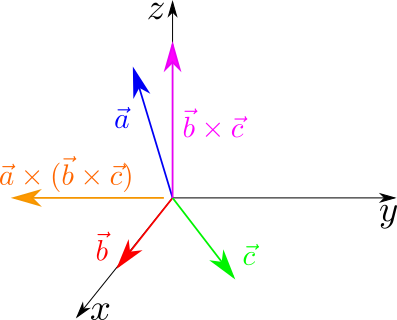
\includegraphics[width=2.2in]
{differ-geo/bac-cab.png}
\caption{Pictorial representation of
BAC minus CAB identity: $\veca \times(\vecb \times \vecc)= \vecb(\veca\cdot\vecc)-
\vecc(\veca\cdot\vecb) $
}
\label{fig-bac-cab-1}
\end{figure}

\begin{claim}
\beq
\nabla
\times
(\nabla \times \vecc)=
\nabla(\nabla\cdot \vecc)-
\nabla^2 \vecc
\eeq

It follows that the Laplacian can
be decomposed into
a sum of a gradient 
(gradient of the divergence of $\vecc$) and
a double cross product
(circulation of circulation of $\vecc$)

\beq
\nabla^2 \vecc
=
\nabla(\nabla\cdot \vecc)
-
\nabla\times
(\nabla \times \vecc)
\eeq

\end{claim}
\proof

\qed

The definition of the
Hodge Laplacian $\Delta$
is a generalization
of this decomposition to p-forms



The {\bf Laplace-Beltrami operator (generalized Laplacian)
$\Delta$} is defined 
as  follows
when it acts on p-forms 
of degree $p$:
\beq
\left\{
\begin{array}{l}
\Delta_p: \wedge_p(M)\rarrow \wedge_p(M)
\\
\Delta_p = d_{p-1}d^\dag_{p-1}+
d^\dag_p d_p
\end{array}
\right.
\eeq

Note that

\beqa
\Delta_p &=&d_{p-1} d^\dag_{p-1}+  d^\dag_p d_p
\\
&=&
d_{p-1}
s_{p-1}
\star_{n-p+1}
d_{n-p}
\star_{p}
+
s_p
\star_{n-p}
d_{n-p-1}
\star_{p+1} d_p
\\
&=&
s_{p-1} (d\star d \star) +
s_p (\star d \star d)
\\
&=&
s_p\left[
(-1)^n
(d\star d \star) +
(\star d \star d)
\right]
\eeqa



Examples
\begin{itemize} 
\item 0-forms

For $n=3$
and an orthonormal coordinate t-basis,
if $f(\rvr)$ is a 0-form

\beqa
\Delta f(\vecr)
&=& \left[\cancel{d d^\dag }+  d^\dag d\right] f
\\
&=&s_1\star d \star \left[\partial_1f \ul{dx} +\cdots\right]
\\
&=&s_1
\star d\left[
\partial_1 f \ul{dy\wedge dz}
+ \cdots\right]
\\
&=&s_1
\star \left[
\nabla^2f \ul{dx \wedge dy \wedge dz}
\right]
\\
&=&s_1
\nabla^2 f
\eeqa
For $n=3$, $s_1=1$
\item 1-forms

For $n=3$ and a 1-form $\pform{\omega}{}=\sum_i \omega_i \pform{dx^i}{}
$

\beqa
d d^\dag \omega_i \ul{dx^i}
&=& s_1
d \star d \star  [\omega_1\ul{dx}+\cdots]
\\
&=& s_1
d \star d[ \omega_1  \ul{dy\wedge dz}+ \cdots]
\\
&=& s_1
d \star [ \partial^i\omega_i   \ul{dx\wedge dy\wedge dz}]
\\
&=& s_1
d \partial^i\omega_i   
\\
&=& s_1
\partial_j
\partial^i \omega_i \ul{dx^j}
\eeqa
so

\beq
[d d^\dag \ul{\omega}]^\sharp= s_1
\nabla (\nabla\cdot (\ul{\omega})^\sharp)
\eeq

\beqa
d^\dag d\omega_i \ul{dx^i}
&=&d^\dag d\left[\omega_1 \ul{dx}+ \cdots\right]
\\
&=&
d^\dag
\left[
(\partial_2\omega_3-\partial_3\omega_2)
\ul{dy\wedge dz}
+\cdots
\right]
\\
&=&s_2
\star d \left[
(\partial_2\omega_3-\partial_3\omega_2)
\ul{dx}
+\cdots
\right]
\\
&=& s_2
\star \left[
(\partial_2 A_3-
\partial_3 A_2) 
\ul{dy\wedge dz}
+\cdots
\right]
\\
&=& s_2
\left[
(\partial_2 A_3-
\partial_3 A_2) 
\ul{dx}
+\cdots
\right]
\eeqa
where 
\beq
A_1 =(\partial_2\omega_3-\partial_3\omega_2)
=
(\nabla\times \omega^\sharp)_1
\eeq
For $n=3$, $s_1=+1$ and $s_2=-1$

\end{itemize}

\begin{claim}
For any p-form $\pform{c}{p}$,
assuming a \Rien metric 

\beq
d\ul{c}=d^\dagger \ul{c}=0
\quad \text{iff}\quad
\Delta \ul{c}=0 
\eeq

\end{claim}
\proof

The $\implies$ direction is obvious
from the definition of $\Delta$.
To prove the converse, note 
the following.

\Rien matrix implies  positive definite inner product.

\beqa
\av{\ul{c}, \Delta \ul{c}}
&=&
\av{\ul{c},
dd^\dag\ul{c}}
+
\av{\ul{c},
d^\dag d\ul{c}}
\\
&=&
\av{d^\dag \ul{c},
d^\dag \ul{c}}
+
\av{d \ul{c},
d \ul{c}}
\\
&=&
\norm{d^\dag \ul{c}}^2
+
\norm{d \ul{c}}^2
\eeqa
Thus

\beq
\Delta\ul{c}
=0
\implies 
d\ul{c}=d^\dag \ul{c}=0
\eeq
assuming the inner product is 
positive definite.

\qed

The last claim fails for a non-\Rien 
metric such as the Lorentz metric.
Laplacians and Hodge theory (see Section \ref{sec-hodge})
behave differently 
in non-\Rien theories.

\subsection{Integration, Stokes' Theorem}

\beq
\ul{d^3 x}= \ul{dx}\wedge\ul{dy}\wedge\ul{dz}
\eeq

If 
\beq
d\vecr =\Delta x \hat{x}
+ \Delta y \hat{y}
+\Delta z \hat{z}
\eeq
then

\beq
\int
f(\vecr)\ul{d^3 x}(d\vecr)
=\int f(\vecr)\Delta x\; \Delta y \; \Delta z
\eeq
Similarly, one can define

\beq
\ul{d^2x}= \ul{dx}\wedge\ul{dy}
\eeq

\beq
\ul{d^1x} = \ul{dx}
\eeq

Stokes' theorem
\beq
\int_U d\pform{\omega}{p}
=
\int_{\partial U}\pform{\omega}{p}
\label{eq-stokes-dif-forms}
\eeq

\beq
\underbrace{\iint\cdots\int}_{\text{$p+1$ times}} d \pform{\omega}{p}
=
\underbrace{\iint\cdots\int}_{\text{$p$ times}}\pform{\omega}{p}
\eeq


\begin{claim}
Stokes' Theorem
Eq.(\ref{eq-stokes-dif-forms}) implies
\beq
\iiint_V\; dV
\nabla\cdot \vec{F}=
\iint_{\partial V}
d\vec{S}\cdot
\vec{F}
\quad\text{(Divergence Theorem)}
\eeq

\beq
\iint_Sd\vec{S}\cdot
\nabla\times \vec{F}
=
\oint_C d\vecr \cdot\vec{F}
\quad
\text{(Curl Theorem)}
\eeq
\end{claim}
\proof

\beq
\vec{F}= [F_1, F_2, F_3]
\eeq

\beq
\ul{\omega}=
F_1 \ul{dx}
+ F_2 \ul{dy}
+
F_3 \ul{dz}
\eeq

\beq
\ul{d\omega}=
[\nabla \times \vec{F}]_1 \ul{dy}\wedge
\ul{dz}
+ (231) + (312)
\eeq
Thus, applying Stokes'
theorem
to $d\ul{\omega}$ leads to
the Curl
Theorem.



\beq
\star\ul{\omega}=
F_1 \ul{dy}\wedge\ul{dz}
+
F_2 \ul{dz}\wedge\ul{dx}
+
F_3 \ul{dx}\wedge\ul{dy}
\eeq

\beq
d\star\ul{\omega}=
\nabla\cdot \vec{F}
\ul{dx}\wedge
\ul{dy}\wedge
\ul{dz}
\eeq
Thus, applying Stokes'
theorem
to $d\star\ul{\omega}$ leads to
the Divergence
Theorem.

\qed




\subsection{Hodge Decomposition}
\label{sec-hodge}


\begin{claim}(Helmholtz decomposition)

For any well behaved vector field $\vec{F}:\RR^3\rarrow \RR^3$, there exists functions $\phi:\RR^3\rarrow \RR$ ,
$\vec{A}:\RR^3\rarrow \RR^3$
and $\vec{H}:\RR^3\rarrow \RR^3$ such that
$\vec{F}$
can be decomposed into a sum of 3 parts, a gradient, a curl,
and a harmonic function:

\beq
\vec{F}= \nabla \phi +
\nabla \times \vec{A} + \vec{H}
\eeq
where

\beq
\nabla^2 \vec{H}=0
\eeq
\end{claim}
\proof
\qed


The operators $d^\dag$ (adjoint derivative) and $\Delta$ (Hodge Laplacian)
are defined in Section \ref{sec-laplacians}

\begin{claim}(Hodge Decomposition)

For any well behaved p-form
$\pform{\omega}{p}$,
there exist p-forms 
$\pform{\alp}{p-1}$,
$\pform{\beta}{p+1}$
and $\pform{c}{p}$
such that
$\pform{\omega}{p}$ can be decomposed
as follows:

\beq
\pform{\omega}{p}=
\underbrace{d\pform{\alp}{p-1}}_{
=\pform{a}{p}, \text{ exact part}}\quad
+\quad
\underbrace{d^\dagger \pform{\beta}{p+1}}_
{=\pform{b}{p}, \text{ coexact part}}
\quad
+
\underbrace{\pform{c}{p}}_{\text{
harmonic part}}
\eeq
where

\beq
\Delta \pform{c}{p}=0
\eeq

\end{claim}
\proof
\qed

\begin{claim}
In the Hodge decomposition,

\beq
\bcen
\xymatrix{
&\rva
\ar@{-}[dl]|{\av{\rva, \rvb}=0}
\ar@{-}[dr]|{\av{\rva, \rvc}=0}
\\
\rvb
\ar@{-}[rr]|{\av{\rvb, \rvc}=0}
&
&\rvc
}
\ecen
\quad\quad
\left\{
\begin{array}{l}
\av{\rva, \rvb}=0
\\
\av{\rva, \rvc}=0
\\
\av{\rvb, \rvc}=0
\end{array}
\right.
\eeq
\end{claim}
\proof

\beq
\av{\rva, \rvb}=
\av{d\ul{\alp}, d^\dagger \ul{\beta}}
=
\av{\ul{\alp}, d^\dag d^\dag \ul{\beta}}=0
\eeq

\beq
\av{\rva, \rvc}=
\av{d\ul{\alp}, \rvc}=
\av{\ul{\alp}, d^\dagger \rvc}=0
\eeq

\beq
\av{\rvb, \rvc}=
\av{d^\dag\ul{\beta}, \rvc}=
\av{\ul{\beta}, d \rvc}=0
\eeq

\qed

The Hodge theory is intimately
connected to the topology of the manifold (how many holes it has, etc.)

Examples
\begin{enumerate}
\item 
Consider polar coordinates $(r, \theta)$ with $M=\RR^2-\{(0,0)\}=$ punctured plane.

We need punctured plane because 
polar coordinates
not well defined at the origin. $\theta$ not ell defined at $r=0$.

\beq
\star \ul{dr}=
r\ul{d\theta},
\quad
\star \ul{d\theta}=
-\;\frac{1}{r}
\ul{dr}
\eeq

\beq
\star \star \ul{dr}=
-\ul{dr}
\eeq
$(-1)^{p(n-1)}=
(-1)^{1(1)}=-1$


\beq
\pform{\omega}{}
=
\pform{d\alp}{}
+ 
\star(\pform{b}{})
+ c \pform{d\theta}{}
\eeq
where $c$ is an arbitrary constant
that arises because the gradient 
$\alp$ is defined only up to $c \theta$

\beq
d^\dag \star \ul{b}=
\star d \star\star \ul{b}=0
\eeq

\beq
\ul{d\alp}=
\alp_r \ul{dr} 
+
\alp_\theta \ul{d\theta}
\eeq

\beq
\ul{b}=
b_r \ul{dr} 
+
b_\theta \ul{d\theta}
\eeq

\beq
\star \ul{b}=
b_r(r\ul{d\theta})
+ b_\theta \left(
-\;\frac{1}{r}\ul{dr}\right)
\eeq

Therefore

\beq
\ul{\omega}=f(r, \theta)\ul{d\theta}=
\left(
\alp_r -\;\frac{b_\theta}{r}
\right)\ul{dr}
+
(\alp_\theta 
+ rb_r+c)\ul{d\theta}
\eeq


\begin{subequations}
\beq
\alp_r -\frac{b_\theta}{r}=0
\eeq

\beq
\alp_\theta + rb_r + c=f
\eeq
\label{eq-alp-b}
\end{subequations}
Eqs.(\ref{eq-alp-b})
must be solved simultaneously for
$(\alp_r, \alp_\theta)$
and $(b_r, b_\theta)$.
This requires 
that we stipulated 
boundary conditions
because the manifold $M$ is not
compact.

Here is an approximate
solution assuming
$\alp_r \approx 0$:

\beq
\pform{\omega}{}=
f(r, \theta)\pform
{d\theta}{}
\eeq
find the 
Hodge decomposition 
of $\ul{\omega}$.

Let $(\vece_1, \vece_2)=(\hat{r}, \hat{\theta})$
and $(\ul{\theta^1},
\ul{\theta^2})=
(\ul{dr}, r\ul{d\theta})$.


\beq
\av{f}(r)=
\frac{1}{2\pi}
\int_0^{2\pi}d\theta \; f(r, \theta)
\eeq

\beq
\delta f = f-\av{f}
\eeq

\beq
\alp_0(r, \theta)=
\int_{0}^\theta d\theta'\;
\delta f(r, \theta')
\quad \text{ for $\theta\in [0, 2\pi]$}
\eeq
Since $\alp(r, 0)=\alp_0(r, 2\pi)=0$,
define $\alp(r, \theta)$ for all $\theta\in \RR$
to be  periodic
in $\theta$ with period $2\pi$.







\beq
d\alp =
\partial_r \alp dr
+
\delta f(r, \theta)d\theta
\eeq

\beq
f(r, \theta)d\theta=
d\alp-\partial_r \alp dr
+
\av{f}(r)
d\theta
\eeq

\beqa
\ul{\omega}&=&
f(r, \theta)\ul{d\theta}
\\
&=&
\ul{d\alp}-\partial_r \alp \ul{dr}
+
\av{f}(r)\ul{d\theta}
\eeqa


\beq
b'(r)
=\frac{\av{f}(r)}{r}
 \eeq

\beq
\star \ul{db}=
\star[b'(r)\ul{dr}]=
rb'(r)\ul{d\theta}=
\av{f}(r)
\ul{d\theta}
\eeq

Since $\partial_r \alp\approx 0$,
\beq
\ul{\omega}\approx
\underbrace{d[\ul{\alp}-c\theta]}_{\text{exact part}}\quad 
+\underbrace{ \star \ul{db}}_{\text{coexact part}}
+ \underbrace{c\ul{d\theta}}_{\text{harmonic part}}
\eeq
Note that the harmonic part 
contains the cut discontinuity 
and thus contains the
topology information.

\beq
\oint_{r=R}d\theta = 2\pi
\eeq

\item $\ul{d\theta}$ properties for 
polar coordinates on punctured plane

\begin{claim}
This
\begin{center}
\begin{tabular}{|l|l|}
\hline
\rowcolor[HTML]{FFFE65} 
$(\cdot)=\ul{d\theta}$ & True everywhere on punctured plane? \\ \hline
$d(\cdot)=0$ (closed) & Yes \\ \hline
$d^\dag(\cdot)=0$ (co-closed) & Yes \\ \hline
$\Delta(\cdot)=0$ (harmonic) & Yes \\ \hline
$(\cdot)=d\ul{\alp}$ (exact) & true locally but not globally \\ \hline
$(\cdot)=d^\dag\ul{\beta}$ (co-exact)& Yes \\ \hline
\end{tabular}
\end{center}
\end{claim}
\proof

$d(\ul{d\theta})=0$ from $d^2=0$

\beq
d^\dagger (\ul{d\theta})
=\star d \star \ul{d\theta}
=
\star d\left(
-\frac{1}{r}\ul{dr}\right)
=0
\eeq

\beq
\Delta(\ul{d\theta}) = \left[d d^\dagger + d^\dag d\right]\ul{d\theta}=0
\eeq
Let 

\beq
\ul{\beta}=-\ln(r)
\ul{dr}\wedge
\ul{d\theta}
\eeq
Then

\beq
d^\dag\ul{d\beta}=
-\star d\star [-\ln(r)
\ul{dr}\wedge
\ul{d\theta}]=-
\star d[\ln(r)]=-
\star \frac{1}{r}
\ul{dr}
=\ul{d\theta}
\eeq


\qed





\end{enumerate}



\subsection{Frobenius Theorem}
\hrule
Fluid mechanics, simple example

\beq
\vecv = x \hat{y} + a\hat{z}
\eeq

\beq
\nabla \times \vecv = 
\left|
\begin{array}{ccc}
\hat{x} &\hat{y}&\hat{z}
\\
\partial_1 &\partial_2 &\partial_3
\\
0 & x & a
\end{array}
\right|
= \hat{z}
\eeq

\beq
\vecv\cdot (\nabla \times \vecv)= 
\hat{z}\cdot [x \hat{y} +a \hat{z}] = a
\eeq

For a  fluid, $\nabla \times \vecv$ is called
the {\bf vorticity} and 
$\vecv \cdot (\nabla\times \vecv)$
is called the
{\bf helicity}. 
Flows with non-zero helicity 
can occur in Nature and be solutions
of Navier-Stokes equation.
No viscosity or turbulence
is required to have them.

Note that when $a=0$, $\nabla \times \vecv$ is still the same,
but $\vecv\cdot (\nabla \times \vecv)=0$. 
That's because 
non-zero 
$\vecv\cdot (\nabla \times \vecv)$ is impossible to achieve in 2-dim.

\begin{figure}[h!]
\centering
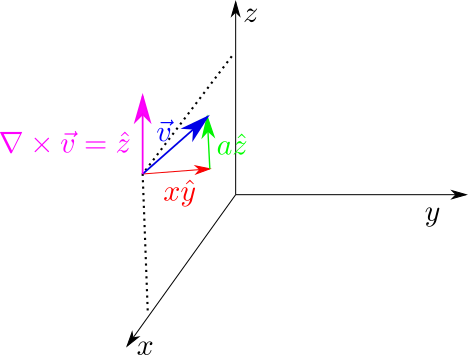
\includegraphics[width=3in]
{differ-geo/helicity-example.png}
\caption{Helicity example}
\label{fig-helicity-example}
\end{figure}



A velocity field is said to be 
{\bf integrable}  if
and only if its streamlines
at every   point $\pi$ 
fall on a plane. 
For non-integrable velocity fields,
if you create a plane at a point $\pi$ with a bunch of streamlines,
then there other streamlines at $\pi$
 will exit the plane.
Frobenius' Theorem for 
3-dim fluid flows is the statement
that a velocity field is integrable
iff it has zero helicity everywhere.
\hrule
Fluid Mechanics, in general

In general

\beq
\vecv\cdot(\nabla \times \vecv)= v_1(\partial_2 v_3 -\partial_3v_2)
+ (231)+ (312)
\eeq
If $\vecv$ is 2-dim, then we can rotate it so that $v_3=\partial_3=0$. Hence, 
the helicity  is zero.

\begin{claim}

\beq
\nabla\times (a\nabla f)=
\nabla a \times \nabla f
\eeq


\end{claim}
\proof

\beqa
\nabla\times (af)=&=&
\left|
\begin{array}{ccc}
\hat{x}& \hat{y}&\hat{z}
\\
\partial_1
&\partial_2
 &\partial_3
\\
a\partial_1f
&a\partial_2f
&a\partial_3 f
\end{array}
\right|
\\
&=&
\left|
\begin{array}{ccc}
\hat{x}& \hat{y}&\hat{z}
\\
\partial_ a
&\partial_2a 
&\partial_3a
\\
\partial_1f
&\partial_2f
&\partial_3 f
\end{array}
\right|
\eeqa
\qed

\begin{claim} 
$\vecv$ has zero helicity iff $\vecv=a\nabla f$
for some functions $a(\vecr)$ and $f(\vecr)$
\end{claim}
\proof

\beqa
\vecv\cdot (\nabla \times \vecv)
&=&
a\nabla f\cdot
(\nabla \times (a\nabla f))
\\
&=&
a\nabla f
\cdot (\nabla a \times \nabla f)
\\
&=&
a
\left|
\begin{array}{ccc}
\partial_1 f
&\partial_2 f
&\partial_3 f
\\
\partial_1 a
&\partial_2 a
&\partial_3 a
\\
\partial_1 f
&\partial_2 f
&\partial_3 f
\end{array}
\right|
\\
&=&
0
\eeqa

\qed

\hrule
Fluid Mechanics, 1-forms

Suppose

\beq
\ul{\omega} = v_1 \ul{dx} + v_2 \ul{dy}
+ v_3 \ul{dz}
\eeq
Then

\beq 
d\ul{\omega}=
(\partial_2 v_3 -\partial_3 v_2)
\ul{dy}\wedge \ul{dz} + (231) + (312)
\eeq

\beqa
\ul{\omega}\wedge
d\ul{\omega} &=&
v_1 (\partial_2 v_3 -\partial_3 v_2)
\ul{dx}\wedge \ul{dy}\wedge \ul{dz}
+ (231) + (312)
\\
&=&
\vecv\cdot(\nabla \times \vecv)
\ul{dx}\wedge \ul{dy}\wedge \ul{dz}
\eeqa
Hence

\beq 
\ul{\omega}\wedge d\ul{\omega}=
0
\quad
\text{iff}\quad
\vecv\cdot (\nabla \times \vecv)=0
\eeq
\hrule
Frobenius Theorem for single and family of 1-forms

The 
Frobenius Theorem (FT)
is a theorem
about 1-forms. 
We first state FT
for a single 1-form.
Then generalize FT to
a family of 1-forms.

\begin{claim}(Frobenius 
Theorem
for single 1-form)

Suppose $\pform{\omega}{}$
is a smooth 1-form in
an $n$ dimensional
manifold $M$.
Suppose

\beq
\ul{\omega}(\vecX)=0
\eeq
for all vector fields $\vecX$.
Define

\beq
D_\pi = \{\vecX\in T_\pi(M):
\ul{\omega}(\vecX)=0\}
\eeq
Then the following statements 
are equivalent
\begin{enumerate}[(a)]
\item $D_\pi$ is a $n-1$ dimensional hypersurface
which deforms continuously as $\pi$ moves.


\item There exist functions $a(\vecX)$ and $f(\vecX)$ such that

\beq
\ul{\omega}(\vecX)=
a(\vecX)\ul{df(\vecX)}
\eeq

\item $\pform{\omega}{}$ satisfies  

\beq
\pform{\omega}{}\wedge
d\pform{\omega}{}=0
\eeq
(always satisfied for $n\leq 2$)

\item For any $\vecX, \vecY \in T_\pi(M)$



\beq
[\vecX_{op}, \vecY_{op}]=0
\eeq 






\end{enumerate}
\end{claim}
\proof
\qed


\begin{claim}(Frobenius 
Theorem
for family of independent 1-forms)

Suppose $\{\pform{\omega^\alp}{}\}_{\alp=1}^n$
is a family of INDEPENDENT  smooth 1-forms in
an $n$ dimensional
manifold $M$.
Suppose

\beq
\ul{\omega^\alp}(\vecX)=0, \quad \text{for } \alp=1, 2, \ldots n
\eeq
for all vector fields $\vecX$.
Define

\beq
D_\pi = \{\vecX\in T_\pi(M):
\ul{\omega^\alp}(\vecX)=0 \text{ for }\alp=1, 2, \ldots n\}
\eeq
Then the following statements 
are equivalent
\begin{enumerate}[(a)]
\item $D_\pi$ is a $n-1$ dimensional hypersurface
which deforms continuously as $\pi$ moves.

\item There exist 
1-forms $\{\pform{\eta^\alp{}}\}$
such that  
\beq
\pform{d\omega^\alp}
{2}=
\sum_\beta
\pform{\eta\indices{^\alp_\beta}}{}
\wedge
\pform{\omega^\beta}{}
\eeq

\end{enumerate}

\end{claim}
\proof

Note that for a single 
1-form, 

\beq
\ul{d\omega}=\ul{\eta}\wedge \ul{\omega}
\implies
\ul{\omega}\wedge \ul{d\omega}=
\ul{\omega}
\wedge
(\ul{\eta}\wedge \ul{\omega})
=0
\eeq
\qed
\hrule
Ideals

A {\bf p-form (PF) ideal} $\cali$ is a set
of p-forms that satisfies the following condition:

\begin{enumerate}
\item $\ul{\alp}\in \cali$ implies 
$\ul{\alp}\wedge \ul{\beta}\in \cali$ for any p-form $
\ul{\beta}$ of any degree.
\end{enumerate}

Ideals are often specified by giving
a set of generators. 
Then the ideal is the set
of all p-forms that have the generators as
\qt{factors} under the wedge product.
For example, 
the ideal with
generators $\{\ul{\theta},\ul{d\theta}\}$ is

\beq
Ideal\{\ul{\theta},\ul{d\theta}\}
=\{\ul{\theta},\quad
 \ul{d\theta}, \quad
f\ul{\theta},\quad
f\ul{d\theta},\quad
\alp\wedge \ul{\theta},\quad
 \ul{\alp}\wedge \ul{d\theta},\quad
\beta\wedge \ul{\theta}\wedge\ul{d\theta},\quad 
\ldots
\}
\eeq
Given an ideal $\cali$ define $d\cali$ by

\beq
d\cali = \{ d\ul{\omega}: \omega\in \cali\}
\eeq
Thus $d\cali$ is the image of $\cali$ under $d$.
We also define the {\bf differential ideal generated by $\cali$} as

\beq
\cali_{diff}= Ideal\{ \cali, d\cali\}
\eeq
\begin{claim}

\beq
\cali =\cali_{diff}\quad
\text{ iff } \quad d\cali \subset \cali
\eeq

\end{claim}
\proof

Suppose $\cali =\cali_{diff}$. Then $d\cali \subset 
\cali_{diff}=\cali$.

Suppose $d\cali\subset \cali$. Then $\cali_{diff}=Ideal\{\cali, d\cali\}=\cali$.

\qed

Frobenius Theorem 
asserts that $D_\pi$ is integrable
iff $\cali=\cali_{diff}$ iff $d\cali\subset \cali$,
where

\beq
\cali = Ideal\{ \pform{\omega^\alp}{}\}_{\alp=1}^n
\eeq


\section{Differential Geometry of General Manifolds}\label{sec-gen-differ-geo}

% Please add the following required packages to your document preamble:
% \usepackage[table,xcdraw]{xcolor}
% Beamer presentation requires \usepackage{colortbl} instead of \usepackage[table,xcdraw]{xcolor}
\begin{table}[h!]
\begin{tabular}{|
>{\columncolor[HTML]{9AFF99}}l |l|}
\hline
def. displacement vector & $\pform{d\vecr}{}= \vece \pform{\theta}{}$ \\ \hline
def. connections & $\pform{d\vece}{} =  \vece \pform{\omega}{}$ \\ \hline
def. torsion (Cartan SE 1) & $\pform{T}{2} = D\pform{\theta}{} =d\pform{\theta}{} + \pform{\omega}{}\wedge \pform{\theta}{}$ \\ \hline
def. curvature (Cartan SE 2) & $\pform{\Omega}{2} = D\pform{\omega}{} = d\pform{\omega}{} +\pform{\omega}{}\wedge\pform{\omega}{}$ \\ \hline
d(torsion) (Bianchi 1) & $D\pform{T}{2} = \pform{\Omega}{2}\wedge \pform{\theta}{}$ \\ \hline
d(curvature) (Bianchi 2) & $D\pform{\Omega}{2} =\pform{\Omega}{2}\wedge \pform{\omega}{}$ \\ \hline
\end{tabular}
\caption{Equations in Cartan Theory, without indices }
\label{tab-Cartan-theory-eqs}
\end{table}

\beq
\xymatrix@C=5pc{
&\pform{\theta}{}\ar[d]|D
&\pform{\omega}{}\ar[d]|D
&
\\
\pform{T}{2}\ar[r]_{-1}
\ar[d]|D
&\Circle{0}
&\Circle{0}
&\pform{\Omega}{2}\ar[l]^{-1}
\ar[d]|D
\\
\Circle{0}
&\pform{\Omega}{2}\wedge\pform{\theta}{}
\ar[l]^{-1}
&\pform{\Omega}{2}\wedge\pform{\omega}{}
\ar[r]_{-1}
&\Circle{0}
}
\eeq

Let

$(\vece_1, \vece_2, \ldots, \vece_n)=$
t-basis


$(\pform{\theta^1}{}, \pform{\theta^2}{} \ldots, \pform{\theta^n}{})=$ dual t-basis. It satisfies

\beq
\ul{\theta^a}
(\vece_b)= \delta^a_b
\eeq

\beq
\pform{d\vecr}{} = \vece_a\pform{\theta^a}{}\quad\text{(displacement vector)}
\eeq

\beq
\pform{\metric}{2}=
\pform{ds^2}{2} =
\pform{\theta^a}{}
\pform{\theta_a}{}
\quad\text{(metric)}
\eeq

$\pform{\omega\indices{^a_b}}{}=$ connection 1-form. It satisfies:

\beq
\pform{d\vece_b}{} =\vece_b
\pform{\omega\indices{^b_a}}{}
\label{eq-de-w-e}
\eeq



SE = Structure Equation

definition of torsion $\ul{T^a}$,
Cartan's First SE
\beq
\pform{T^a}{2} = \pform{d\theta^a}{2} + \pform{\omega\indices{^a_b}}{}\wedge \pform{\theta^b}{}
\eeq

definition of curvature $\ul{\Omega\indices{^a_b}}$,
Cartan's Second SE 

\beq
\pform{\Omega\indices{^a_b}}{2} =\pform{d\omega\indices{^a_b}}{2}
+
\pform{\omega\indices{^a_c}}{}
\wedge
\pform{\omega\indices{^c_b}}{}
\eeq

\begin{claim}(Bianchi Identities)

\beq
\pform{dT^a}{3}=-
\pform{\omega\indices{^a_b}}{}
\wedge
\pform{T^b}{2} 
+
\pform{\Omega\indices{^a_b}}{2}
\wedge
\pform{\theta^b}{}
\quad \text{(First Bianchi Identity)}
\eeq


\beq
\pform{d\Omega\indices{^a_c}}{3}=
-
\pform{\omega\indices{^a_b}}{}
\wedge
\pform{\Omega\indices{^b_c}}{2}
+
\pform{\Omega\indices{^a_b}}{2}
\wedge
\pform{\omega\indices{^b_c}}{}
\quad\text{(Second Bianchi Identity)}
\eeq


\end{claim}
\proof

These identities both
come from applying a $d$ derivative
to Cartan's first and second structure functions.

\beqa
d\ul{T} &=& \cancel{d^2 \ul{\theta}} + (d\ul{\omega})\wedge\ul{\theta}
-\ul{\omega} \wedge d\ul{\theta}
\\
&=&
(d\ul{\omega})\wedge \ul{\theta}
-
\ul{\omega}\wedge
(\ul{T} - \ul{\omega}\wedge \ul{\theta})
\\
&=&
-\ul{\omega} \wedge \ul{T}
+ 
\underbrace{[d\ul{\omega}
+ \ul{\omega}\wedge\ul{\omega}]}_{\ul{\Omega}}
\wedge \ul{\theta}
\eeqa

\beqa
d\ul{\Omega} &=& \cancel{ d^2 \ul{\omega}}
+ (d\ul{\omega})\wedge \ul{\omega}
-  \ul{\omega} \wedge (d\ul{\omega})
\\
&=&
[\ul{\Omega} - \ul{\omega}\wedge \ul{\omega}]\wedge \ul{\omega}
-
\ul{\omega}\wedge [\ul{\Omega} - \ul{\omega}\wedge \ul{\omega}]
\\
&=&
\ul{\Omega} \wedge \ul{\omega} - \ul{\omega} \wedge \ul{\Omega}
\eeqa

\qed

\section{Differential Geometry of Curves}\label{sec-frenet-serret}

{\bf Frenet-Serret} (notice it rhymes) {\bf equations}

Let

$\vecr(s)=$
1-dim curve in 3-dim parametrized by
arc length $s$

$\hatT=$ {\bf tanget unit vector},  tangent to curve at  point $\pi$

$\hatN=|\frac{dT}{ds}|^{-1} \frac{dT}{ds}=$
{\bf principal normal unit vector}, normal to curve at point $\pi$.
Of all the vectors
normal to the 
curve at $\pi$, this is a unique one.

$\hatB=\hatT\times\hatN
=$ {\bf principal binormal unit vector}, normal  to curve at point $\pi$. $\bcen\xymatrix{
&&
\\
&&
\\
\ar[rr]^\hatN
\ar[uu]^\hatB
\ar[dr]_\hatT&&
\\
&&
}\ecen$

$\kappa=$ curvature

$\tau=$ torsion


\beqa
\frac{d\hatB}
{ds}&=&
-\tau \hatN
\\
\frac{d\hatN}
{ds}&=&
\tau\hatB -\kappa\hatT
\\
\frac{d\hatT}
{ds}&=&
\kappa \hatN
\eeqa

\beq
\xymatrix{
\hatB ds
\ar[dr]|<<<<\tau
&\hatN ds\ar[dr]|<<<<\kappa
\ar[dl]|<<<<{-\tau}
&\hatT ds
\ar[dl]|<<<<{-\kappa}
\\
d\hatB
&d\hatN
&d\hatT
}
\eeq

\beq
\hatN=\hatB\times\hatT
\eeq
so

\beqa
\frac{d\hatN}{ds}&=&
\frac{d\hatB}{ds}
\times \hatT
+
\hatB\times
\frac{d\hatT}{ds}
\\
&=&
-\tau  \hatN \times \hatT
+
\hatB \times \kappa \hatN
\\
&=&
\tau \hatB - \kappa \hatT
\eeqa


\beq
\left[
\begin{array}{c}
d\hatT
\\
d\hatN
\\
d\hatB
\end{array}
\right]
=
\left[
\begin{array}{ccc}
0
&\kappa ds
&0
\\
-\kappa ds
&0
&\tau ds
\\
0
&-\tau ds
&0
\\
\end{array}
\right]
\left[
\begin{array}{c}
\hatT
\\
\hatN
\\
\hatB
\end{array}
\right]
\eeq

\beq
\underbrace{
\left[
\begin{array}{c}
\pform{d\vece_1}{}
\\
\pform{d\vece_2}{}
\\
\pform{d\vece_3}{}
\end{array}
\right]
}_{\pform{dE}{}}
=
-
\underbrace{\left[
\begin{array}{ccc}
0
&\pform{\omega_{12}}{}
&0
\\
\pform{\omega_{21}}{}
&0
&\pform{\omega_{23}}{}
\\
0
&\pform{\omega_{32}}{}
&0
\\
\end{array}
\right]}_{\pform{W}{}}
\underbrace{\left[
\begin{array}{c}
\vece_1
\\
\vece_2
\\
\vece_3
\end{array}
\right]}_{E}
\eeq

\beq
\pform{d\vece_a}{}=
-\pform{\omega_{ab}}{}\vece_b
\eeq

\begin{figure}[h!]
\centering
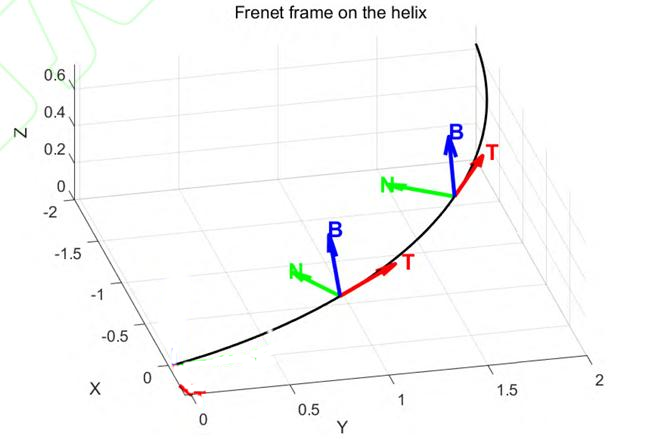
\includegraphics[width=4in]
{differ-geo/helix.png}
\caption{Picture of a circular helix with moving frame
$\hatT, \hatN, \hatB$}
\label{fig-helix}
\end{figure}

Circular helix
\beq
\vecr(s)= (a\cos(s), a\sin(s), bs)
\eeq

straight line: $a=0$

circle: $b=0$, $a=R$

\beq
\vecr\;'(s)=
(-a\sin(s), a \cos(s), b)
\eeq

\beq
\hatT = \frac{\vecr\;'}{|\vecr\;'|}
=
\frac{1}{\sqrt{a^2 + b^2}}(-a\sin(s), a\cos(s), b)
\eeq

\beq
\kappa =\left|
\frac{d\hatT}{ds}
\right|
\quad \rarrow \quad
\hatN = \frac{1}{\kappa}
\frac{d\hatT}{ds}
\quad \rarrow \quad
\hatB = \hatT \times \hatN
\quad \rarrow \quad
\tau = - \left|
\frac{d\hatB}{ds}
\right|
\eeq


% Please add the following required packages to your document preamble:
% \usepackage[table,xcdraw]{xcolor}
% Beamer presentation requires \usepackage{colortbl} instead of \usepackage[table,xcdraw]{xcolor}
\begin{table}[h!]
\begin{tabular}{|l|l|l|}
\hline
\rowcolor[HTML]{FFFC9E}
Curve & Curvature $\kappa$ & Torsion $\tau$ \\ \hline
Straight line & $0$ & $0$ \\ \hline
Circle & $1/R$ & $0$ \\ \hline
Helix & $a/(a^2 + b^2)$ & $b/(a^2 + b^2)$ \\ \hline
\end{tabular}
\caption{Curvature and Torsion for some curves in $\RR^3$}
\label{tab-frenet}
\end{table}

\section{Differential Geometry of Surfaces}

Let

$(\hate_1, \hate_2)=$
orthonormal t-basis



 $(\hate_1, \hate_2, \hat{n})=$ orthonormal
t-basis, $\hat{n}$ normal to tangent plane

$(\pform{\theta^1}{}, \pform{\theta^2}{})=$ dual t-basis. 

Everything covered in Section 
\ref{sec-gen-differ-geo} applies to
this case of 2-dim surfaces in $\RR^3$.
In this case, the indices $a, b,\ldots$ 
range over $\{1, 2\}$
For Euclidean space ($\RR^3$), we don't have
to distinguish between upper and lower indices.

The definition of the connection 1-forms
$\ul{\omega_{ab}}$ takes the form
\beq
\left[
\begin{array}{c}
\ul{d\hate_1}
\\
\ul{d\hate_2}
\end{array}
\right]=
-
\left[
\begin{array}{cc}
0 &\ul{\omega_{12}}
\\
-\ul{\omega_{12}}&0
\end{array}
\right]
\left[
\begin{array}{c}
\hate_1
\\
\hate_2
\end{array}
\right]
\eeq
\beq
\pform{d\hate_a}{}=
-\pform{\omega_{ab}}{}\hate_b
\eeq
The  matrix of connections
$\ul{\omega}=[\ul{\omega_{ab}}]$ must be anti-symmetric because the t-basis $(\hate_1, \hate_2)$
is orthonormal.


From the first SE,
assuming zero torsion,

\beq
\ul{d\theta_a}=
-
\ul{\omega_{ab}}\wedge \ul{\theta_b}
\eeq

\beq
\boxed
{\ul{d\theta_1}=-\ul{\omega_{12}}\wedge\theta_2,\quad
\ul{d\theta_2}=\ul{\omega_{12}}\wedge\theta_1}
\eeq

From the second SE,

\beq
\ul{\Omega_{12}}=
\ul{d\omega_{12}} +
\cancel{\ul{\omega_{1c}}
\wedge
\ul{\omega_{c2}}}^0
\label{eq-Omega-dw}
\eeq

Note that $(\ul{\theta_1},\ul{\theta_2})$ is a basis for the dual
tangent vector space so we must have

\beq
\pform{\omega_{12}}{}=
A \pform{\theta_1}{} + B\pform{\theta_2}{}
\label{eq-omega12-t1-t2}
\eeq

From
Eq.(\ref{eq-Omega-dw})
and  Eq.(\ref{eq-omega12-t1-t2}), we must have

\beq
\ul{\Omega_{12}}=
K \ul{\omega_1}
\wedge\ul{\omega_2}
\eeq
for some constant $K$.
$K$ is called the {\bf Gaussian  curvature (scalar curvature)}.


\beq
\boxed
{\ul{\Omega_{12}}=\ul{d\omega_{12}}= K
\ul{\theta_1}\wedge\ul{\theta_2}}
\label{eq-K-theta1-theta2}
\eeq

\beq
\xymatrix@C=1pc{
\pform{\omega_{12}}{}
\ar[d]|{d}
\\
\pform{d\omega_{12}}{2}
\ar[d]^1
&
\pform{\theta_1}{}\wedge
\pform{\theta_2}{}
\ar[dl]|K
\\
\Circle{0}
}\quad
\xymatrix@C=1pc{
\pform{\theta_1}{}
\ar[d]|d
&&
&\pform{\theta_2}{}
\ar[d]|d
\\
\pform{d\theta_1}{2}
\ar[d]^1
&
\pform{\omega_{12}}{}\wedge
\pform{\theta_1}{}
\ar[drr]|{1}
&
\pform{\omega_{12}}{}\wedge
\pform{\theta_2}{}
\ar[dll]|{-1}
&
\pform{d\theta_2}{2}
\ar[d]^1
\\
\Circle{0}
&&
&\Circle{0}
}
\eeq

GB from point of view of p-forms

From Eq.(\ref{eq-K-theta1-theta2})
\beq
d\pform{\omega_{12}}{1}= K \pform{\theta_1}{}
\wedge \pform{\theta_2}{}=
K \pform{d^2 x}{2}
\eeq

\beq
\iint_M dA \; K\rarrow
\iint_M d\ul{\omega_{12}}
\eeq

Stokes theorem

\beq
\iint_M \ul{d\omega}=
\int_{\partial M}
\ul{\omega}
\eeq

\beq
\omega\rarrow \omega + \ul{d\alp}
\eeq


Examples
\begin{enumerate}
\item $S^2=\{(x,y, z)
\mid x^2 + y^2 + z^2 = R^2\}$, surface of sphere in 3-dim

\begin{figure}[h!]
\centering
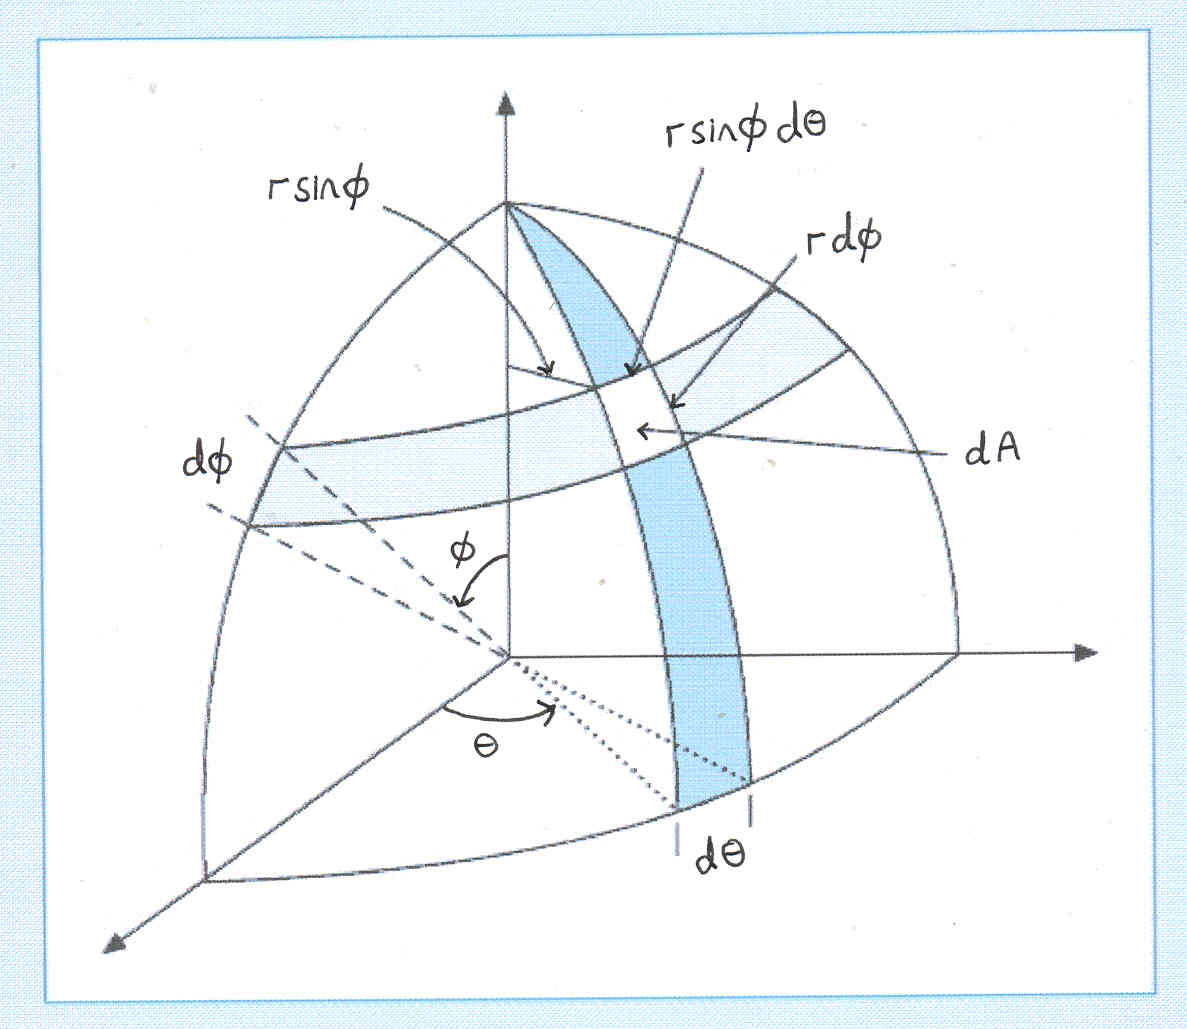
\includegraphics[width=3.5in]
{differ-geo/polar-3d.jpg}
\caption{Polar coordinates in 3-dim.}
\label{fig-polar-3d}
\end{figure}

parametrization

\beq
\left\{
\begin{array}{l}
x=R\sin(\phi)\cos(\theta)
\\
y=R\sin(\phi)\sin(\theta)
\\
z=R\cos(\phi)
\end{array}
\right.
\eeq
for $\phi\in[0,\pi]$
and $\theta \in [0, 2\pi]$.

Instead of using the coordinate t-basis


\beq
d\vecr =
Rd\phi\hat{\phi}
+
R\sin(\phi)d\theta\hat{\theta}
\eeq

At the surface $S$, the metric is
\beq
\AT{(ds)^2}{S} =
R^2(d\phi)^2 +
R^2 \sin^2(\phi)
(d\theta)^2
\eeq

\begin{claim}
If
\beq
\ul{\theta_1}=
R\ul{d\phi},
\quad
\hate_1 =\hat{\phi}
\eeq

\beq
\ul{\theta_2}=
R\sin(\phi)
\ul{d\theta},
\quad
\hate_2 =\hat{\theta}
\eeq
then

\beq
\ul{\omega_{12}}
=
-\;\frac{\cot(\phi)}{R}\ul{\theta_2}
=-\cos(\phi)
\ul{d\theta}
\eeq


\beq
\ul{d\theta_1}=0\eeq

\beq
\ul{d\theta_2}
=
\frac{\cot(\phi)}{R}
\ul{\theta_1}
\wedge
\ul{\theta_2}
=
R \cos(\phi)
\ul{d\phi}
\wedge \ul{d\theta}
\eeq

\beq
\ul{\Omega_{12}}
=\ul{d\omega_{12}}
=
\underbrace{\frac{1}{R^2}}_{K}
\ul{\theta_1}
\wedge\ul{\theta_2}
=\sin(\phi)
\ul{d\phi}
\wedge
\ul{d\theta}
\eeq
\end{claim}
\proof

Zero torsion
so

\beq
\ul{d\theta_a}
+
\ul{\omega_{ab}}
\wedge \ul{\theta_b}=0
\eeq

\beqa
\cancel{\ul{d\theta_1}}^0
+
\ul{\omega_{12}}
\wedge
\ul{\theta}_2
=0
\\
\ul{d\theta_2}
-
\ul{\omega_{12}}
\wedge
\ul{\theta}_1
=0
\eeqa

First equation implies

\beq
\ul{\omega_{12}}=A \ul{\theta_1}
\eeq
Second equation
can be used to solve for $A$.


\beq
\frac{\cot(\phi)}{R}
\ul{\theta_1}
\wedge\ul{\theta_2}+
A\ul{\theta_1}
\wedge \ul{\theta_2}=0
\implies
A = -\;\frac{\cot(\phi)}{R}
\eeq

\qed
\item {\bf Mobius strip}.
Its curvature
changes as one moves on the surface but its torsion is zero.
\item {\bf Helicoid.}
Its curvature
changes as one moves on the surface but its torsion is zero.

\item {\bf crystal dislocations}

Neither $S^2$, nor the Mobius strip nor a Helicoid
have torsion. Here
is an example of a surface
in 3-dim that does.
Basically, it's like a Helicoid, but instead of
growing uniformly in the $z$-direction, it
sallies forth in the $z$-direction but before going around a full turn,
it changes its mind and comes
back to where it started.

\begin{figure}[h!]
\centering
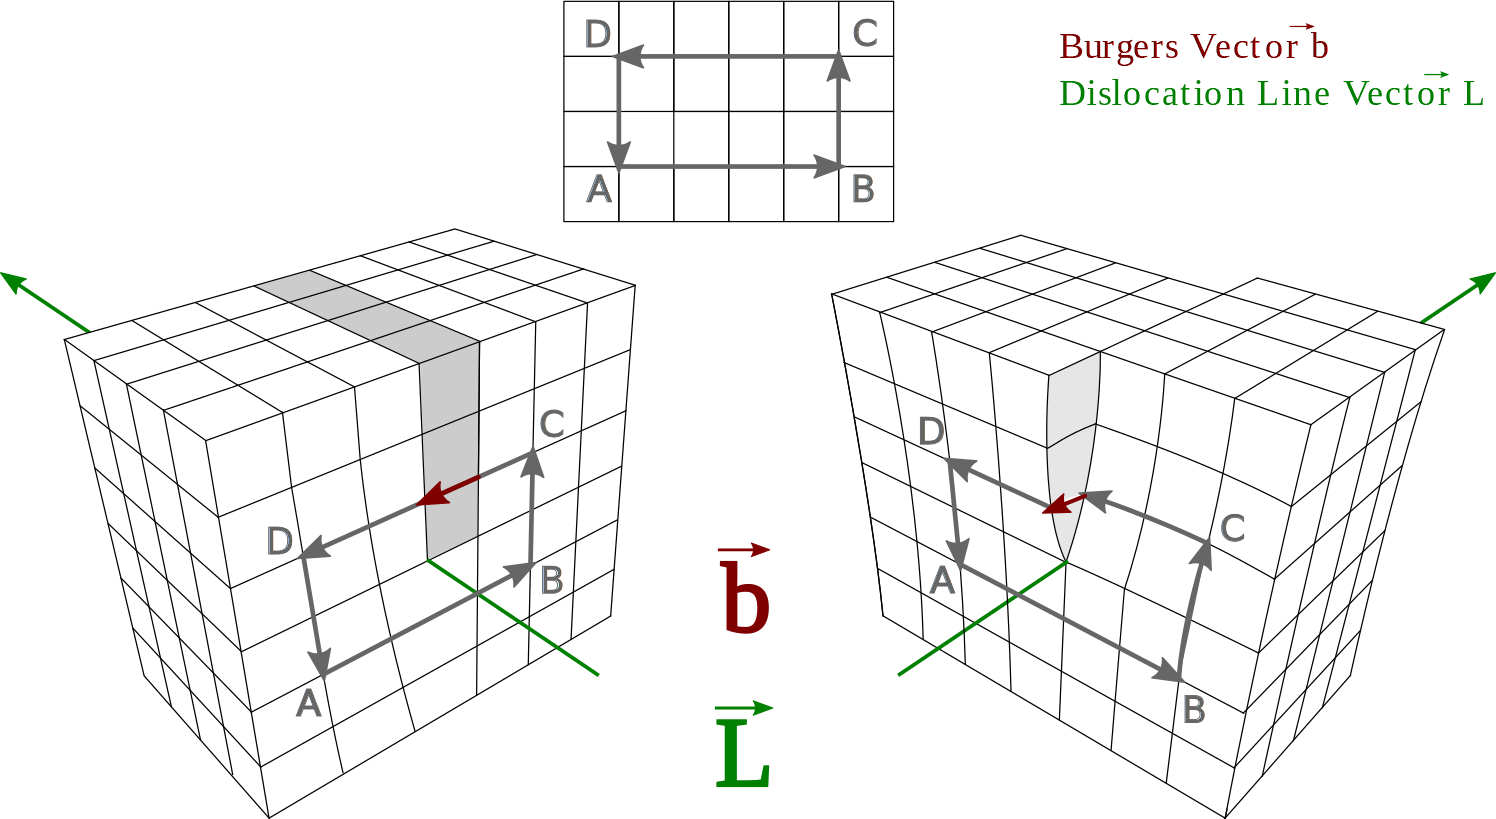
\includegraphics[width=5in]
{differ-geo/burgers_vector.png}
\caption{Burgers vector in an edge dislocation (left) and in a screw dislocation (right). The edge dislocation can be imagined as the introduction of a half plane (gray boxes) that does not fit the crystal symmetry. The screw dislocation can be imagined as cut and shear operation along a half plane.
(This image and caption by Martin Fleck comes
from the Wikipedia article
on Burgers Vector
*******
%\cite{wiki-burgers}
)}
\label{fig-burgers-vector}
\end{figure}

$\vecr\rarrow \vecr + \vec{u}(\vecr)$ (in 3-dim)

For a perfect crystal,

\beq
\oint_C d\vec{u}=0
\eeq
If the
crystal has a dislocation,
 $\vec{u}$
averaged over the closed loop may be non-zero.
{\bf Burger's vector} $\vec{b}$

\beq
\vec{b}=
\oint_C d\vec{u}
\eeq


\beq
b_i =
\oint_C
\pder{u_i}{x^j}dx^j
\eeq

Applying Stokes' theorem, this line integral can be converted to
a surface integral
over a curl. If the vector normal to surface $S$ is $n_i$, then

\beq b_i=
\int
\int_S
\eps_{jkl}
\frac{\partial^2 u_i}{
\partial x^k \partial x^l
}n_j dS
\eeq

\beq
\alp_{ij}=
\eps_{jkl}
\pder{\beta_{il}}{x^k},
\quad
\beta_{il}=
\pder{u_i}{x^l}
\eeq
$\alp_{ij}=$ {\bf dislocation
density tensor},
$\beta_{il}=$
{\bf distortion tensor
}

\beq
b_i =
\iint_S \alp_{ij}n_j dS
\eeq
In Cartan  notation,

\beq
\vec{u}\rarrow \pform{\theta^a}{}=
e^a_i
\pform{dx^i}{}
\eeq

\beq
\pform{T^a}{2
}
=\pform{d\theta^a}{}+
\pform{\omega\indices{^a_b}}
{}\wedge
\pform{\theta^b}{}
\eeq
When dealing with crystals, it's possible to choose a connection
called the Weitzenb\"{o}ck (teleparallel) connection, for which
$\ul{\omega\indices{^a_b}}=0$.\footnote{If the
teleparallel connection is not being used, one must
include the contribution
of $\ul{\omega\indices{^a_b}}
\wedge \ul{\theta^b}$
in the calculation of  Burger's vector.} Then

\beq
b^a=
\oint_C \pform{\theta^a}{}
\eeq
By Stokes' theorem,

\beq
b^a =
\int_S
\pform{T^a}{2}
\eeq

\end{enumerate}

\subsection{Orientability}
\begin{figure}[h!]
\centering
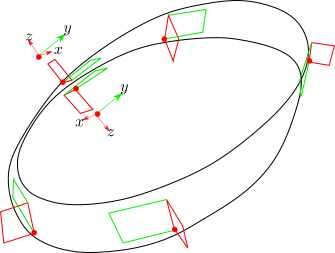
\includegraphics[width=3.1in]
{differ-geo/mobius-coords.png}
\caption{After one pass around a Mobius
strip, a right-handed triad $(x,y, z)$ evolves to a different triad  wherein
the $x$ and $z$ directions
are reversed, but $y$
direction is the same.
The triad stays right handed but it is not the
same as the original as is required for continuity.}
\label{fig-mobius-coords}
\end{figure}

\begin{figure}[h!]
\centering
\includegraphics[width=3in]
{differ-geo/Mobius-plus-disk.png}
\caption{
Red arrows, green arrows and green points are identified.  This figure shows that glueing the single edge of a Mobius strip to the single edge of a disk gives 
$RP^2$.
The identified green dots 
on the right hand side are essentially the border of the disk shrunk to 2 identified points.}
\label{fig-mobius-plus-disk}
\end{figure}



Given a set 
of coordinates $(x^1, x^2, x^3, \dots x^n)$ is a particular order of those coordinates 
which we 
define as a positive
orientation.
Any odd (resp., even) permutation 
of that order is called 
a negative (resp., positive)
orientation.
In $\RR^3$,
the Cartesian coordinates $(x,y,z)$
defined by the right-hand rule,
are said to
have a positive orientation.

An {\bf orientable
surface}
is a surface 
for which one can define define an orientation and that 
orientation is preserved
as we travel on the surface.
Not all surfaces are orientable.
For example,
the 
Mobius strip
is not orientable.
(See Fig.\ref{fig-mobius-coords})
The projective plane isn't either.

The {\bf projective plane ($RP^2$)}
is the surface $S^2$ of a sphere with 
antipodal points identified.
Hence

\beq
RP^2 =
\{ \{x, -x\}: x\in S^2\}
\eeq

If we define the equivalence relation $\sim$ over $S^2$ so that for every $x, y\in S^2$, $x\sim y$ if $y=-x$, then 
$RP^2=\{[x]: x\in S^2 
\}$.
The set of 
equivalence classes over a set $A$ is often denoted by
$A/ \sim$. Hence $RP^2=
S^2/\sim$. Note that the division sign here  means something totally different 
from the division sign 
used to indicate a quotient space in group theory, $RP^2\cong S^2/\{-1, 1\}$, where $\cong$ means isomorphic.
To make the notation $A/\sim$ more group theory like,
replace $A/\sim$ by $A/[x]_\sim$, were 
 $[x]_\sim$ is any equivalence
class of $\sim$ in $A$.

A second way way of defining 
$RP^2$
is to define it as 
the set  of all the lines through the origin.
Or a the set of equivalence  classes of vectors that lie on a line through the origin.
For every $x\in \RR^3-\{0\} $, let

\beq
L_x =\{ax: a\in \RR-\{0\}\}
\eeq
Then

\beq
RP^n
=
\{
L_x: x\in \RR^n -\{ 0\}
\}
\eeq

A third way of defining 
$RP^2$ as a hemisphere 
with opposite ends of its boundary identified.
But a hemisphere 
can be flatten to a disc $D^2$, so $RP^2$ is also isomorphic to
a disk with
opposite ends of every diameter identified.

The Mobius strip and the
projective plane are
closely connected. 
Notice that a Mobius
strip really has one edge,
although at first it appears to have two edges, if you go around it in your mind, you realize that 
after each revolution, the top edge piece flows into the bottom edge piece which flows into the \qt{top}edge, and so on. Fig.\ref
{fig-mobius-plus-disk} shows that glueing the single edge of a Mobius strip to the single edge of a disk gives 
$RP^2$.  Topologists represent glueing surfaces by a hash. Hence,

\beq
M^2\# D^2\cong RP^2
\eeq

\subsection{Gauss Theorema Egregium}

\hrule
Gauss

Start by parametrizing the surface

\beq
\vecr = \vecr(u_1, u_2)
\eeq
$(u_1, u_2)=(u,v)$


\beq
d\vecr = \partial_{u_1}\vecr\; du_1 +
\partial_{u_2}\vecr\; du_2
\eeq
Latin indices 
will range over
$\{1,2\} $.
$\partial_i =\partial_{u_i}$
Einstein summation convention

\beq
d\vecr = 
\underbrace{\partial_i \vecr}_{=\vecpder{u_i}=\ket{i}}
\;
du_i
\eeq

\beq
\underbrace
{\partial_1 \vecr
\cdot \partial_1\vecr}_
{\gauE}=E,
\quad
\underbrace{\partial_1 \vecr
\cdot \partial_2\vecr}
_{\gauF}=F,
\quad
\underbrace{\partial_2 \vecr
\cdot \partial_2\vecr}_{\gauG}=G
\eeq

\beq
\left[
\begin{array}{cc}
\av{1|1} &\av{1|2}
\\
\av{2|1}&\av{2|2}
\end{array}
\right]
=
\left[
\begin{array}{cc}
E &F
\\
F&G
\end{array}
\right]
\eeq

First fundamental quadratic form
\beq
Q_I= d\vecr\cdot d\vecr = du_i du_j \av{i|j}
\eeq

$\hat{n}=\ket{3}$ unit vector
perpendicular to the surface

\beq
\av{3|3}=1,
\quad
\av{3|1}=\av{3|2}=0
\eeq

\beq
\underbrace{\partial_1\partial_1\vecr}_
{\ket{11}}
 = 
\Gamma^1_{11}
\ket{1}
+\Gamma^2_{11}
\ket{2} 
+ e\ket{3}
=
\Gamma^i_{11}\ket{i}+ e \ket{3}
\eeq

\beq
\underbrace{\partial_1\partial_2\vecr}_
{\ket{12}} 
= 
\Gamma^1_{12}
\ket{1}
+\Gamma^2_{12}
\ket{2} 
+ f
c\ket{3}
=
\Gamma^i_{12}\ket{i}+ f \ket{3}
\eeq

\beq
\underbrace{\partial_2\partial_2\vecr}
_{\ket{22}}
 = 
\Gamma^1_{22}
\ket{1}
+\Gamma^2_{22}
\ket{2} 
+ g\ket{3}
=
\Gamma^i_{22}\ket{i}+ g \ket{3}
\eeq
Christoffel symbols

\beq
\Gamma^k_{ij}= \av{k|ij}
\eeq

\beq
\gaue=e,
\quad
\gauf=f,
\quad
\gaug=g
\eeq

\beq
\left[
\begin{array}{cc}
\av{3|11} &\av{3|12}
\\
\av{3|21}&\av{3|22}
\end{array}
\right]
=
\left[
\begin{array}{cc}
e &f
\\
f&g
\end{array}
\right]
\eeq

Second Fundamental quadratic form
\beq
Q_{II}= du_i du_j \av{3|ij}
\eeq
\hrule
Cartan 


\begin{table}[h!]
\begin{tabular}{|l|l|l|}
\hline
 & \cellcolor[HTML]{FFCCC9}Gauss & \cellcolor[HTML]{FFCCC9}Cartan \\ \hline
\cellcolor[HTML]{9AFF99}t-basis and normal unit vector & $(\ket{1}, \ket{2}, \ket{3})$ & $(\hate_1, \hate_2, \hatn)$ \\ \hline
\cellcolor[HTML]{9AFF99}dual t-basis and normal unit vector& $(du_1, du_2, du_3)$ & $(\ul{\theta_1}, 
\ul{\theta_2},
\ul{\theta_3})$ \\ \hline
\cellcolor[HTML]{9AFF99}connections & $\Gamma^k_{ij}=\av{k|ij}, \quad \av{3|ij}$ 
& $\ul{\omega_{12}},\quad
 \ul{\omega_{23}},\quad
 \ul{\omega_{13}}$ \\ \hline
\end{tabular}
\caption{Comparison between Gauss and Cartan formalism for studying surfaces}
\label{tab-gauss-cartan-compare}
\end{table}

\begin{figure}[h!]
\centering
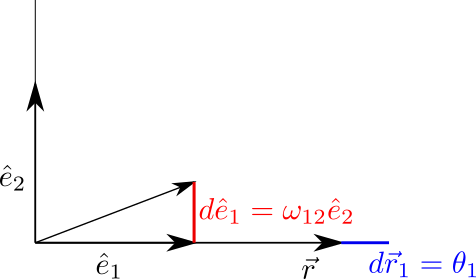
\includegraphics[width=3in]
{differ-geo/dr1-de1.png}
\caption{
Geometrical significance of
$\omega_{ij}$ and $\theta_i$
as differentials, before they
are turned into 1-forms.
It's fine to replace an equation between 1-forms to an equation between
differentials. Cartan
language augments the language of 1-forms by adding p-forms
of degree $>1$.
We also try visualize the 2-forms $\ul{d\theta_i}$ 
and $\ul{d\omega_{ij}}$.}
\label{fig-dr1-de1}
\end{figure}


Basis $(\ket{1}, \ket{2}, \ket{3})$ is  not 
orthonormal.
Cartan chooses 
orthonormal basis
$(\hate_1, \hate_2, \hate_3)$
where

\beq
\hate_3 =\hatn=\ket{3}
\eeq

\beq
\pform{d\vecr}{} =\pform{ \theta_1}
{}\hate_1
+
\pform{ \theta_2}
{}\hate_2
=
\pform{\theta_i}{}\hate_i
\eeq

\beq
\ul{d\vecr}\cdot \ul{d\vecr}=
\ul{\theta_1}^2 +\ul{\theta_2}^2
\eeq

\beq
Q_I = du_idu_j \av{i|j}= \theta_i\theta_i
\eeq

\beq
\hate_1 = \frac{\ket{1}}
{\sqrt{\gauE}}
\eeq

\beq
\hate_2=
\frac{
\gauE\ket{2}-
\gauF\ket{1}
}{D
\sqrt{
\gauE
}
}
\eeq

\beq
\hate_3= \ket{3}
\eeq
where

\beq
D =\sqrt{\gauE\gauG-\gauF^2
}
\eeq

\beq
\theta_i = \hate_i\cdot d\vecr
\eeq

\beq
\theta_1 = 
\frac{1}{\sqrt{\gauE}}
\left(
\gauE du_1
+
\gauF du_2
\right)=
\frac{
\av{1|i}du_i
}{\sqrt{\gauE}}
\eeq

\beq
\theta_2=
\frac{D du_2}
{\sqrt{\gauE}}
\eeq






\beq
\pform{d\vecr}{} =
\pform{\theta_1}{}\hate_1
+
\pform{\theta_2}{}\hate_2
=
\pform{\theta_i}{}\hate_i
\eeq

\beq
\hate_i\cdot \hate_j=\delta_{ij}
\eeq


\beq
\left[
\begin{array}{c}
\pform{d\hate_1}{}
\\
\pform{d\hate_2}{}
\\
\pform{d\hatn}{}
\end{array}
\right]
=
\left[
\begin{array}{ccc}
0
&\pform{\omega_{12}}{}
&\pform{\omega_{13}}{}
\\
-\pform{\omega_{12}}{}
&0
&\pform{\omega_{23}}{}
\\
-\pform{\omega_{13}}{}
&-\pform{\omega_{23}}{}
&0
\end{array}
\right]
\left[
\begin{array}{c}
{\hate_1}{}
\\
{\hate_2}{}
\\
{\hatn}{}
\end{array}
\right]
\eeq


\begin{align}
0&= d^2\ul{\vecr}
\\
&=
d(\hate_i\ul{\theta_i})
\\
&=
\hate_i \ul{d\theta_i}
+
\ul{d\hate_i}\wedge \ul{\theta_i}
\\
&=
\hate_i \ul{d\theta_i}
+
\left[
\ul{\omega_{12}}\hate_2
+\ul{\omega_{13}}\hatn
\right]\wedge \ul{\theta_1}
+\left[
-\ul{\omega_{12}}\hate_1
+\ul{\omega_{23}}\hatn
\right]\wedge \ul{\theta_2}
\\
&=
\hate_i \ul{d\theta_i}
+
\hate_1\left[
-\ul{\omega_{12}}\wedge\ul{\theta_2}
\right]
+\hate_2
\left[
\ul{\omega_{12}}\wedge \ul{\theta_1}
\right]
+\hatn
\left[
\ul{\omega_{13}}\wedge\ul{\theta_1}
+
\ul{\omega_{23}}\wedge \ul{\theta_2}
\right]
\end{align}

\beqa
\ul{d\theta_1} &=&
\ul{\omega_{12}}\wedge \ul{\theta_2}
\\
\ul{d\theta_2} &=&
-\ul{\omega_{12}}\wedge\ul{\theta_1}
\\
0&=&
\ul{\omega_{13}}\wedge\ul{\theta_1}
+
\ul{\omega_{23}}\wedge \ul{\theta_2}
\eeqa
Cartan's first structure equations with zero torsion.'


\beq
\left[
\begin{array}{c}
\ul{\omega_{13}}
\\
\ul{\omega_{23}}
\end{array}
\right]
=
\underbrace
{\left[
\begin{array}{cc}
h_{11}&h_{12}
\\
h_{21}&h_{22}
\end{array}
\right]}_\calh
\left[
\begin{array}{c}
\ul{\theta_1}
\\
\ul{\theta_2}
\end{array}
\right]
\eeq
\beq
\ul{\omega_{13}}\wedge\ul{\theta_1}
+
\ul{\omega_{21}}\wedge \ul{\theta_2}
\implies
h_{12}=h_{21}
\eeq





$\alp, \beta\in \{1,2,3\}$
\beq
\ul{d\hate_\alp}= \ul{\omega_{\alp\beta}}
\hate_\beta
\eeq

\beqa 
0&=&
d\ul{d\hate_\alp}
\\
&=&
d(\ul{\omega_{\alp\beta}})\hate_\beta
+
\ul{d\hate_\mu}
\wedge  \ul{\omega_{\alp\mu}}
\\
&=&
d(\ul{\omega_{\alp\beta}})\hate_\beta
+
\ul{\omega_{\mu\beta}}\hate_\beta
\wedge 
\omega_{\alp\mu}
\eeqa

\beq
\ul{d\omega_{\alp\beta}}=
\ul{\omega_{\alp\mu}}\wedge \ul{\omega_{\mu\beta}}
\eeq

\beq
\ul{d\omega_{12}}= \ul{\omega_{13}}
\wedge \ul{\omega_{32}}
\eeq

Definition of curvature $K$
\beq
\ul{d\omega_{12}}=
K\ul{\theta_1}
\wedge
\ul{\theta_2}
\eeq

\begin{claim}(Gauss Theorema Egregium, Version 1)

\beq
\ul{d\omega_{12}}=
K\ul{\theta_1}
\wedge
\ul{\theta_2}=
\ul{\omega_{13}}
\wedge \ul{\omega_{32}}
\eeq

\end{claim}
\proof

\qed



\begin{claim}(Second Fundamental Form)

\beq
\ul{Q_{II}}=
\ul{\theta_i}h_{ij}\ul{\theta_j}=
\ul{du_i}\av{i|j}\ul{du_j}
\eeq

\end{claim}
\proof

\beq
\ul{du_i}(\vecpder{u^i})=\delta_{ij},\quad
\ul{\theta_i}(\hate_j)=\delta_{ij}
\eeq

Define
\beq
\ul{Q_{II}}(\vecX, \vecY)=
\hatn\cdot \nabla_\vecX(\vecY)
\eeq

First assume 

\beq
\vecX =X^i\hate_i,
\quad \vecY =Y^i\hate_i
\eeq

Then

\beqa
\ul{Q_{II}}(\vecX, \vecY)
&=&
X^i \hatn\cdot\nabla_{\vece_i}
(Y^j \hate_j)
\\
&=&
X^i\hatn\cdot
\left[
\cancel{(\nabla_{\hate_i}Y^j)}\hate_j
+
Y^j\nabla_{\hate_i}\hate_j
\right]
\\
&=&
X^i Y^j \hatn\cdot\nabla_{\hate_i}\hate_j
\eeqa

\beq
\nabla_\vecX \hate_i=
\ul{d\hate_i}(\vecX) =
\ul{\omega_{ij}}(\vecX)\hate_j +
\ul{\omega_{i3}}(\vecX)\hat{n}
\eeq

\beq
\hatn\cdot\nabla_\vecX \hate_i=\ul{\omega_{i3}}(\vecX)
\eeq


\beq
\ul{Q_{II}}(\vecX, \vecY)
=Y^j\ul{\omega_{j3}}(\vecX)
\eeq

\beq
\ul{\omega_{j3}} (\vecX)= h_{ji}\ul{\theta_i}(\vecX)=
h_{ji}X^i
\eeq

\beq
\ul{Q_{II}}(\vecX, \vecY)=
X^ih_{ij}Y^j =
\ul{\theta_i}(\vecX)h_{ij}\ul{\theta_j}(\vecY)
\eeq

Next assume

\beq
\hate_i \rarrow \vecpder{u^i},
\quad \ul{\theta_i}\rarrow \ul{du_i}
\eeq

\beq
\ul{Q_{II}}(\vecX, \vecY)
=Y^j\ul{\omega_{j3}}(\vecX)
\eeq

\beq
\ul{\omega_{j3}} (\vecX)= \av{j|i}\ul{du_i}(\vecX)=
\av{j|i}X^i
\eeq

\beq
\ul{Q_{II}}(\vecX, \vecY)=
X^i\av{ij}Y^j =
\ul{du_i}(\vecX)\av{i|j}\ul{du_j}(\vecY)
\eeq
\qed


\begin{claim}(Gauss Theorema Egregium, Version 2)

\beq
\frac{eg-f^2}
{EG-F^2}=
h_{11}h_{22}-h_{12}^2
=
K
\eeq

\end{claim}
\proof

\beq
\left[
\begin{array}{c}
\ul{\theta_1}
\\
\ul{\theta_2}
\end{array}
\right]=
\cala
\left[
\begin{array}{c}
\ul{du_1}
\\
\ul{du_2}
\end{array}
\right]
\eeq

\beq
Q_I
=
\left[
\begin{array}{cc}
\ul{du_1}
&
\ul{du_2}
\end{array}
\right]
\calq_I
\left[
\begin{array}{c}
\ul{du_1}
\\
\ul{du_2}
\end{array}
\right]=
\left[
\begin{array}{cc}
\ul{\theta_1}
&
\ul{\theta_2}
\end{array}
\right]
\underbrace{(\cala^{-1})^T\calq_I \cala^{-1}}_{1}
\left[
\begin{array}{c}
\ul{\theta_1}
\\
\ul{\theta_2}
\end{array}
\right]
\eeq

\beq
\calq_I = [\av{i|j}],\quad
\calq_I=\cala^T\cala
=\text{metric at surface in $(u_1, u_2)$ coords}
\eeq


\beq
Q_{II}
=
\left[
\begin{array}{cc}
\ul{du_1}
&
\ul{du_2}
\end{array}
\right]
\calq_{II}
\left[
\begin{array}{c}
\ul{du_1}
\\
\ul{du_2}
\end{array}
\right]=
\left[
\begin{array}{cc}
\ul{\theta_1}
&
\ul{\theta_2}
\end{array}
\right]
\underbrace{(\cala^{-1})^T \calq_{II} \cala^{-1}}_{\calh}
\left[
\begin{array}{c}
\ul{\theta_1}
\\
\ul{\theta_2}
\end{array}
\right]
\eeq

\beq
\calq_{II} = [\av{3|ij}],\quad
\calq_{II} =
\cala^T\calh\cala
\eeq

\beq
\frac
{\det{\calq_{II}}}
{\det{\calq_{I}}}=
\det\calh = K
\eeq

\beq
\frac{eg-f^2}
{EG-F^2}=
h_{11}h_{22}-h_{12}^2
=
K
\eeq

\qed


\begin{claim}
If 
\beq
\omega_{12}=
A_idu_i
\eeq
then

\beq
A_1 = 
\frac{\gauE \partial_2\gauE
-
2\gauE \partial_1\gauF
+
\gauF \partial_1\gauE}
{
2\gauE D
}
\eeq

\beq
A_2 =
\frac{-\gauE \partial_1\gauG
+ \gauF \partial_2 \gauE
}
{
2\gauE D}
\eeq
\end{claim}
\proof
\beq
\left\{
\begin{array}{ll}
\theta_1 = \frac{\av{1|i}du_i}
{\sqrt{\gauE}}
&(a)
\\
\theta_2 =
\frac{Ddu_2}
{\sqrt{\gauE}}
&(b)
\\
\omega_{12}= A_i du_i
& (c)
\\
\ul{d\theta_1}=
-\ul{\omega_{12}}
\wedge \ul{\theta_2}
&(d)
\\
\ul{d\theta_2}=
\ul{\omega_{12}}\wedge
\ul{\theta_1}
& (e)
\end{array}
\right.
\eeq
Take the exterior derivative of $\theta_1$ given by $(a)$. Plug that and $(b), (c)$ into $(d)$ to get $A_1$.

Take the exterior derivative of $\theta_2$
given by $(b)$. Plug that and $(a), (c)$ into $(e)$ to get $A_2$.
\qed



\subsection{Euler Characteristic}
\begin{table}[h!]
\begin{tabular}{|l|l|l|l|l|}
\hline
 & \cellcolor[HTML]{FFCCC9}$F$ & \cellcolor[HTML]{FFCCC9}$V$ & \cellcolor[HTML]{FFCCC9}$E$ & \cellcolor[HTML]{FFCCC9}$\chi$ \\ \hline
\cellcolor[HTML]{9AFF99}triangle & 1 & 3 & 3 & 1 \\ \hline
\cellcolor[HTML]{9AFF99}square & 1 & 4 & 4 & 1 \\ \hline
\cellcolor[HTML]{9AFF99}pentagon & 1 & 5 & 5 & 1 \\ \hline
\cellcolor[HTML]{9AFF99}hexagon & 1 & 6 & 6 & 1 \\ \hline
\cellcolor[HTML]{9AFF99}cube & 6 & 8 & 12 & 2 \\ \hline
\cellcolor[HTML]{9AFF99}tetrahedron & 4 & 4 & 6 & 2 \\ \hline
\cellcolor[HTML]{9AFF99}\begin{tabular}[c]{@{}l@{}}Surface of Sphere ($S^2$)\\ (see Fig.\ref{fig-polygons-surfaces})\end{tabular} & 4 & 4 & 6 & 2 \\ \hline
\cellcolor[HTML]{9AFF99}\begin{tabular}[c]{@{}l@{}}Torus ($T^2$)\\ (see Fig.\ref{fig-polygons-surfaces})\end{tabular} & 4 & 4 & 6 & 2 \\ \hline
\cellcolor[HTML]{9AFF99}\begin{tabular}[c]{@{}l@{}}Projective Plane ($RP^2$)\\ (see Fig.\ref{fig-polygons-surfaces})\end{tabular} & 6/2 & 8/2 &12/2 & 1\\ \hline
\cellcolor[HTML]{9AFF99}\begin{tabular}[c]{@{}l@{}}Mobius Strip ($M^2$)\\ (see Fig.\ref{fig-polygons-surfaces})\end{tabular} & 3 & 4 & 7 & 0 \\ \hline
\end{tabular}
\caption{Euler Characteristic $\chi$ for various surfaces computed from polygonalization}
\label{tab-my-tabletab-euler-examples}
\end{table}

The {\bf Euler Characteristic} 
of a 2-dim surface $M$
built from polygonal facets  
is defined as 

\beq
\chi(M) = V+ F-E
\eeq
(remember, only $E$ makes a negative contribution)
where 

$V=$ number of vertices of $M$

$F=$ number of faces of $M$

$E=$ number of edges of $M$

$M$ is often taken to be embedded in $\RR^2$ or $\RR^3$ but that is not necessary or relevant.

A smooth surface can be approximated by polygonal facets
to calculate its $\chi$.
See Table \ref{tab-my-tabletab-euler-examples}.

How fine this polygonalization  is does not change $\chi$ 
because it's a topological property.
As evidence of this, note that $\chi$ for a triangle
is invariant under the addition
of an extra edge or vertex. (See Fig.\ref{fig-euler-chi})

\begin{figure}[h!]
\centering
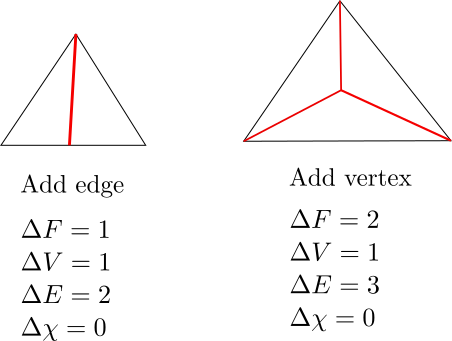
\includegraphics[width=2.5in]
{differ-geo/euler-chi.png}
\caption{Change in Euler characteristic of
a plane triangle when an extra edge or
vertex is added.}
\label{fig-euler-chi}
\end{figure}

\begin{figure}[h!]
\centering
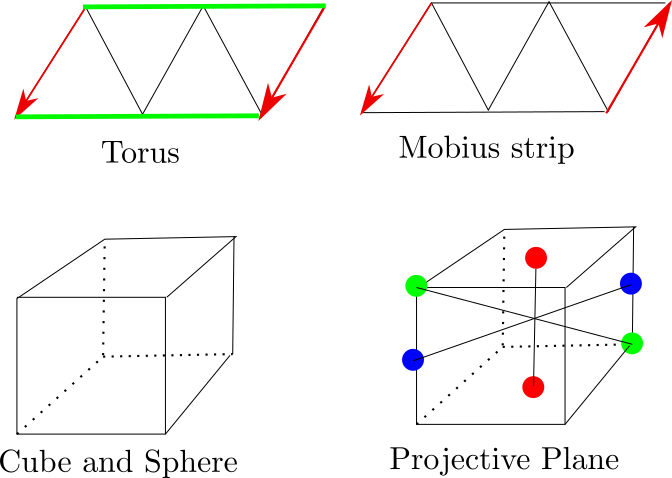
\includegraphics[width=3.1in]
{differ-geo/polygons-surfaces.png}
\caption{Polygonalizations 
of various surfaces. $S^2$ is approximated by
a cube: crude but good enough. Edges and points
that have same color (red, green or blue)
are identified.}
\label{fig-polygons-surfaces}
\end{figure}

The {\bf genus $g$} of an orientable surface is the number
of holes (same as the number of handles) in the surface.

Genus is not defined 
for non-orientable surfaces.
For them, we 
have instead
the {\bf number of crosscaps $k$}.
$RP^2$ has one crosscap.
Surfaces with
$k>1$  crosscaps (like the Klein bottle which has $k=2$) can be viewed as constructed from $k$ copies of $RP^2$. 
A surface can have both holes and crosscaps, but one can convert each hole
into 2 crosscaps. Hence, if $k>0$, we normally assume $g=0$.




From a subdiscipline
of Differential Geometry called 
Cohomology, it is possible
to prove a deep connection between 
the Euler characteristic $\chi$
of a manifold, and its
genus $g$
or crosscaps $k$.

\beq
\chi(M)=
\left\{
\begin{array}{ll}
2- 2g& \text{if $M$ is orientable}
\\
2-k&\text{otherwise}
\end{array}
\right.
\label{eq-chi-from-g-k}
\eeq

See Table 
\ref{chi-orientable-non-orientable} for
examples of Eq.(\ref{eq-chi-from-g-k}).
\begin{table}[h!]
\begin{tabular}{|l|l|l|l|l|l|l|}
\hline
 & \cellcolor[HTML]{FFCCC9}$\chi$ & \cellcolor[HTML]{FFCCC9}orientable? & \cellcolor[HTML]{FFCCC9}$g$ & \cellcolor[HTML]{FFCCC9}$2-2g$ & \cellcolor[HTML]{FFCCC9}$k$ & \cellcolor[HTML]{FFCCC9}$2-k$ \\ \hline
\cellcolor[HTML]{9AFF99}$S^2$ & 2 & yes & 0 & 2 & NA & NA \\ \hline
\cellcolor[HTML]{9AFF99}$T^2$ & 0 & yes & 1 & 0 & NA & NA \\ \hline
\cellcolor[HTML]{9AFF99}$RP^2$ & 1 & no & NA & NA & 1 & 1 \\ \hline
\cellcolor[HTML]{9AFF99}Kein bottle & 0 & no & NA & NA & 2 & 0 \\ \hline
\end{tabular}
\caption{Euler characteristic $\chi$ compared to $2-2g$ (orientable) or $2-k$ (non-orientable).NA=not applicable}
\label{chi-orientable-non-orientable}
\end{table}



\subsection{Gauss Bonnet Theorem}

The Gauss-Bonnet (GB)
theorem says that the
Gaussian curvature $K$ integrated over an entire \ul{orientable} 2-dim manifold $M$ (i.e., an orientable surface)
gives a topological invariant. It's very
important that 
the surface be orientable
as the GB theorem does not
work
for non-orientable surfaces. 

We will state the Gauss-Bonnet (GB)
for 3 cases, in order of increasing complexity
\begin{enumerate}
\item GB for closed surface (i.e., surface, like 
a sphere or a torus,
with no boundaries)

\item GB for a surface with a smooth boundary

\item GB for a surface with piecewise smooth 
boundary with a finite number of corners

Let 


\end{enumerate}

\begin{claim}(GB for closed surface $M$)

\beq
\iint_M dA \; K = 2\pi \chi(M)
\eeq
\end{claim} 
\proof
Motivation (not rigorous proof)

Suppose we compute the normal unit vector $\hat{n}(\pi)$
at every point $\pi$ of the manifold $M$, and then we translate 
that vector to $S^2$, the surface
of a sphere with unit radius.
The translation should be done without changing the direction of $\hat{n}(\pi)$, so that the
new vector $\phi(\hat{n}(\pi))$ aligns with a line through the
origin of the sphere.
This is called the {\bf Gauss map.} 

Next notice that the
solid angle $dA$ subtended by
a neighborhood of $\pi$ in the 
manifold $M$ is related by
the solid angle $d\Omega$ 
in the neighborhood of $\phi(\hat{n}(\pi))$, by

\beq
K dA = d\Omega
\eeq
If $M=S^2$, this gives

\beq
\iint_{S^2}dA\; K = \int_{S^2}d\Omega = 4\pi
\eeq
This is agrees with the KB 
theorem because $\chi(S^2)=2$.

Actual proof:

Suppose $M$ 
is a compact, smooth,
orientable surface with no boundaries

First, triangularize $M$
into a fine mesh of
geodesics triangles (i.e. triangles whose edges are 
]geodesics of $M$)

Two steps: 
\begin{enumerate}

\item Apply Stokes Theorem to
a single geodesic triangle $\Delta$

Let
$(\hate_1, \hate_2)$ be an
orthonormal basis at point
$\pi$ of tangent plane

\beq
\ul{d\hate_1}=\ul{\omega}\hate_2,
\quad
\ul{d\hate_2}=-\ul{\omega}\hate_1
\eeq

\beq
\ul{d\omega}= A_1 \ul{\theta_1}
+
A_2 \ul{\theta_2}
\eeq

\beq
\ul{d\omega}=
\left[
\partial_1 A_2-\partial_2 A_1
\right]
\ul{\theta_1}\wedge\ul{\theta_2}
\eeq

\beq
\vecX = X^1\hate_1 + X^2\hate_2
\eeq

\beq
\ul{d\omega}(\vecX)
=
-K \underbrace{\ul{\theta_1}(\Delta X_1\hate_1)
\wedge\ul{\theta_2}(\Delta X_2\hate_2)}_{dA}
\eeq

\beq
\iint_\Delta dA\; K=
-\iint_\Delta \ul{d\omega}(\vecX)=
-\oint_{\partial \Delta}
\ul{\omega}(\vecX)
\eeq

counterclockwise contour

Tangent $\vecT$ to edge

\beq
\vecT = \cos(\phi)\hate_1 +
\sin(\phi)\hate_2
\eeq

Indicate derivatives $d/ds$ by prime

\beq
(\hate_1', \hate_2')=
\omega(\hate_2, -\hate_1)
\eeq

\beqa
\vecT\;'&=&
\left[-\sin(\phi)\phi'
-\omega \sin(\phi)
\right]\hate_1
+ 
\left[
\cos(\phi)\phi'
+\omega \cos(\phi)
\right]\hate_2
\\
&=&
(\phi'+\omega)
\left
[-\sin(\phi)\hate_1
+\cos(\phi)\hate_2
\right]
\eeqa

{\bf geodesic curvature}

\beq
k_g(s) = \phi'(s) +\omega(s)
\eeq
For a geodesic, $k_g=0$ so

\beq
\omega(s)=-\phi'(s)
\eeq

\beq
-\oint_{\partial\Delta}\omega=
\oint_{\partial\Delta }ds\; \phi'(s)=
\sum_{i=1}^3\Delta \phi_i
\eeq

\beq
\iint_\Delta dA\; K=
\sum_{i=1}^3\Delta \phi_i
\eeq

Let 

$\Theta_1, \Theta_2, \Theta_3=$
interior angles of geodesic triangle

$\alp_i=\pi-\Theta_i=$ changes 
in direction of $\vecT$
at each vertex

\beq
\sum_{i=1}^3
(\Delta \phi_i +\alp_i)=2\pi
\eeq

\beq
\sum_{i=1}^3\Delta\phi=-\pi+
\sum_{i=1}^3\Theta_i
\eeq

\beq
\iint_\Delta dA\; K=
-\pi +\sum_{i=1}^3 \Theta_i
\eeq


\item Add contributions of all 
geodesic triangles

\beq
\iint_M dA\; K
=
-\pi F
+\sum_v\sum_{i=1}^3\Theta_i^{(v)}
\eeq

\beq
\sum_v\sum_{i=1}^3\Theta_i^{(v)}=
2\pi V
\eeq

\beq
\iint_M dA\; K=
-\pi F + 2\pi V=
2\pi(V-F/2)
\eeq

Take a tetrahedron as an example. It has four faces and six edges so $E/F= 6/4= 3/2$.
The reason it doesn't have $3(4)=12$ edges is because every edge is shared by two triangles so effectively, the number of edges for all triangles is $12/2=6$. In general, not just for the tetrahedron,

\beq
E/F = 3/2
\eeq

\beq
\chi(M)=V+F-E=
V+F-3/2F=
V-F/2
\eeq

\beq
\iint_M dA\; K= 2\pi\chi(M)
\eeq



\end{enumerate}





\qed



\begin{figure}[h!]
\centering
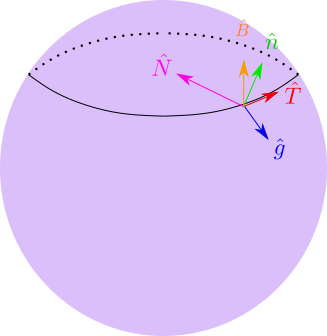
\includegraphics[width=2.5in]
{differ-geo/geo-curvature.png}
\caption{Example
in which
the right handed triads $(\hatT, \hatN, \hatB)$
and $(\hatN, \hat{n}, \hat{g})$ differ.}
\label{fig-geo-curvature}
\end{figure}

Let 

$\hatT=$ unit vector tangent to the boundary
at point $\pi$.

$ds=$ infinitesimal
length of segment at boundary point $\pi$.

$\hat{n}=$
unit vector normal to the surface
at boundary point $\pi$.

$\hat{g}=\hatT\times \hat{n}=$ unit vector
on tangent plane 
of point $\pi$.

$k_n=$ {\bf normal curvature}

$k_g=$ {\bf geodesic curvature}


\beq
\frac{d\hatT}{ds}=
k_g \hat{g}
+ k_n\hat{n}
\eeq


Note that the Frenet-Serret 
equations (see Section \ref{sec-frenet-serret})
use a right handed
triad $(\hatT, \hatN, \hatB)$.
In that case, there 
is no surface. In this case there is.
The right handed triad $(\hatT, \hat{n}, \hat{g})$
is defined with respect to a  surface. The vectors
$(\hatN, \hatB)$
span the same plane
as the vectors $(\hat{n}, \hat{g})$
but they are different orthonormal bases
in general.
In fact, $\hatN\propto k_g\hat{g}+ k_n\hat{n}$.



\begin{claim}(GB for a surface $M$
with a smooth boundary)

\beq
\iint_M dA\;K  
+  \oint_{\partial M}
ds\; k_g
= 2\pi \chi(M)
\eeq
\end{claim} 
\proof
\qed

A piecewise smooth 
boundary with 
a finite number of corners changes direction at the i'th corner by an angle $\alp_i$.
The angles $\alp_i$ 
are called the {\bf exterior turning angles}.
The angles
$\theta_i=\pi-\alp_i$ are called the  {\bf interior angles}.

\begin{claim}(GB for a surface $M$
with a
piecewise smooth boundary
with a finite number of corners)

\beq
\iint_M dA\;K  
+  \sum_i \oint_{\partial M_i}
ds\; k_g
+
\sum_i \alp_i
= 2\pi \chi(M)
\eeq
\end{claim} 
\proof
\qed


It's common to 
apply the GB 
theorem
to a patch $M$ of a larger manifold $M'$
and to choose 
the boundaries of $M$ to be $E$ geodesics.
In that case, $k_g=0$
along all the 
smooth geodesic pieces of the boundary and GB reads

\beq
\iint_MdA\; K=
2\pi\chi(M)
-\pi E + 
\sum_{i=1}^E \theta_i
\eeq



Examples
\begin{enumerate}
\item Let $M$ be a flat triangular region. Then $K=0$,
$\chi(M)=1$ and $E=3$ so we get

\beq
0=2\pi-3\pi +\sum_{i=1}^3 \theta_i
\eeq
As expected,

\beq
\sum_{i=1}^3 \theta_i =\pi
\eeq

\item Consider a flat disk $D^2_R$ of radius $R$.
In this case, $K=0$ so

\beq
\oint_{D^2_R}ds \;k_g= 2\pi\chi
\eeq
$k_g=1/R$
and $\chi=1$ so both sides equal $2\pi$.

\item Consider a Torus $T^2_R$
where $R$ is the radius at the center. 
For $T^2_R$, $\chi=0$ so GB becomes

\beq
\iint_{T^2_R}dA \;K=0
\eeq
Suppose $(r, \phi, \theta)$
are cylindrical coordinates.
The reason for this is because
$T^2_R$ has $K>0$ outside (i.e., for $r>R$),  $K=0$ for $r=R$ and
$K<0$ inside (i.e., for $r<R$)

 
\item Let $S^2_R$ be the surface of a sphere
of radius $R$,
and $M\subset S^2_R$ be a  triangular patch of $S^2_R$ 
 bounded by 3 great circles. In that case,
$\chi(M)=\chi(S^2_R)=2$ and $E=3$. 
Hence we get

\beq
\iint_M dA\; K =\pi + \sum_{i=1}^3
\theta_i
\eeq
Since the curvature of $S^2_R$
equals $1/R^2>0$, this means 

\beq
4\pi \geq \iint_M dA\; K=
\pi +\sum_{i=1}^3 \theta_i
\eeq
so

\beq
3\pi \geq \sum_{i=1}^3 \theta_i
\eeq
Again, this is as expected as 
clearly, if $M$ is 1/8
of $S^2_R$, this inequality is 
saturated.

\end{enumerate}

\section{Fluid Mechanics}


\begin{itemize}

\item coordinates $(x^1, x^2, x^3)=(x,y,z)$


\item velocity

velocity field
\beq
\vecv= v^i \hat{x}_i
\eeq

velocity 1-form
\beq
\pform{\beta}{}=
\vecv\;^\flat =
v_i\pform{dx^i}{}
\eeq

\item circulation
\beq
\Gamma =
\oint_C \vecv\cdot d\vecr = \oint_C \pform{\beta}{}
\eeq

\item vorticity

\beq
\vec{\omega}=\nabla
\times \vecv
\eeq

\beq
\pform{\omega}{2}
=
\pform{d\beta}{2}
\eeq

\beqa
\pform{\omega}{2}
&=&
\frac{1}{2}
\left(
\partial_i v_j
-
\partial_j v_i
\right)
\pform{dx^i}{}
\wedge
\pform{dx^j}{}
\\
&=&
\left(
\partial_2{v_3}-
\partial_3{v_2}
\right)
\pform{dx^2}{}
\wedge
\pform{dx^3}{}
+ (231)+ (312)
\eeqa

\beq
\pform{\omega}{2}=
(\star \;^\flat)(\vec{\omega})
\eeq

\item
volume 3-form

\beq
\pform{d^3 x}{3}=
\pform{\star 1}{3}=
\pform{dx}{}\wedge
\pform{dy}{}\wedge
\pform{dz}{}
\eeq

\item material derivative $\cald$

\beq
\cald  = \partial_t + \vecv\cdot \nabla
\eeq
$\vecv\cdot \nabla$
is  directional derivative.
Thus the material derivative
equals a time derivative plus a directional derivative in the direction of $\vecv$.


\end{itemize}

Stokes' theorem for vorticity

\beq
\oint_C
\vecv\cdot d\vec{r}=
\iint
d\vec{S}\cdot (\nabla\times \vecv)
\eeq

\beq
\oint_{\partial S}\ul{\beta}=
\iint_S \ul{d\beta}
\eeq



incompressible flow

\beq
\nabla\cdot \vecv=0
\eeq


\beqa
d\star \pform{\beta}{}
&=&d\;\left[v^1 \pform{dx^2}{}\wedge\pform{dx^3}{}+
(231)+ (312)\right]
\\
&=&
[\nabla\cdot \vecv] \pform{d^3 x}{3}
\eeqa


\beqa
d\;i_\vecv\;\pform{d^3 x}{3}
&=&d\;\left[v^1 \pform{dx^2}{}\wedge\pform{dx^3}{}+
(231) + (312)\right]
\\
&=&
[\nabla\cdot \vecv] \pform{d^3x}{3}
\eeqa

\beq
d\star \pform{\beta}{} =
d\;i_\vecv\;\pform{d^3x}{3} =0
\eeq

\hrule
Euler's equation
for ideal incompressible fluid

\beq
\partial_t \vecv +
(\vecv \cdot \nabla)
\vecv +
\frac{1}{\rho}\nabla p=0
\eeq

Recall the BAC minus CAB
rule for double cross products

\beq
\veca \times(\vecb \times \vecc)= \vecb(\veca\cdot\vecc)-
\vecc(\veca\cdot\vecb)
\eeq
The following is a generalization to the case where $\vecb=\nabla$.

\begin{figure}[h!]
\centering
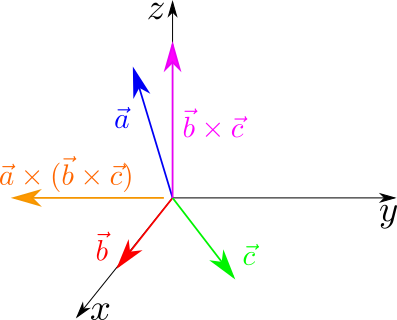
\includegraphics[width=2.2in]
{differ-geo/bac-cab.png}
\caption{Pictorial representation of
BAC minus CAB identity: $\veca \times(\vecb \times \vecc)= \vecb(\veca\cdot\vecc)-
\vecc(\veca\cdot\vecb) $
}
\label{fig-bac-cab-2}
\end{figure}

\begin{claim}

\beq
(\vecv \cdot \nabla)\vecv=
\nabla\left(
\frac{1}{2}|\vecv|^2
\right)
-
\vecv \times  (\nabla \times\vecv)
\eeq
i.e., directional 
derivative of $\vecv$
can be decomposed into 
a gradient and $\vecv$ cross
the  circulation.

\beq
\left[
\vecv\times(\nabla \times \vecv)
\right]_i=
v_j[\partial_i v_j-
\partial_j v_i]
\eeq
\end{claim}
\proof

\beqa
v_1\hat{x}\times (\nabla \times \vecv)
&=&
v_1\hat{x}\times
\left[
\hat{y}(\partial_3 v_1-\partial_1 v_3)
+
\hat{z}(\partial_1 v_2-\partial_2 v_1)
\right]
\\
&=&v_1
\left[\hat{z}(\partial_3 v_1-\partial_1 v_3)
-
\hat{y}(\partial_1 v_2-\partial_2 v_1)
\right]
\\
&=&
v_1
\left[
\hat{z}\partial_3 +\hat{y}\partial_2
\right]v_1
+
v_1\partial_1\left[
-\hat{z}v_3
-\hat{y}v_2
\right]
\\
&=&
v_1 \nabla v_1 -
v_1\partial_1 \vecv
\\
&=&
\nabla \left(
\frac{1}{2}v_1^2\right) -
v_1\partial_1 \vecv
\eeqa
Thus

\beq
\vecv \times  (\nabla \times\vecv)=
\nabla\left(
\frac{1}{2}|\vecv|^2
\right)
-
(\vecv \cdot \nabla)\vecv
\eeq

\beqa
\left[\vecv\times(\nabla \times \vecv)
\right]_i &=&
\partial_i\left(
\frac{1}{2} |\vec{v}|^2\right)
-v_j\partial_j v_i
\\
&=&
v_j[\partial_i v_j-
\partial_j v_i]
\eeqa

This can also
be proved using the identity

\beq
\eps_{pqa}\eps_{amn}=
\delta^{pq}_{mn}-
\delta^{pn}_{qm}
\eeq
as can the BAC minus CAB rule.
\qed


\beq
\partial_t \vecv
-
{\vecv \times  (\nabla \times\vecv)}
+\nabla\left(
\frac{1}{2}|\vecv|^2
\right)
 +
\frac{1}{\rho}\nabla p=0
\eeq

\beq
\left[\vecv\times(\nabla \times \vecv)
\right]_r=
v_j
\left[\partial_r v_j
-\partial_j v_r
\right]
\eeq

\beqa
i_\vecv \pform{\omega}{2}&=&
v_j(\partial_j v_r-
\partial_r v_j)
\pform{dx^r}{}
\\
&=&
-\left[\vecv\times(\nabla \times \vecv)
\right]_r \pform{dx^r}{}
\eeqa

\beq
\Phi = \frac{1}{2}|\vecv|^2
+ \frac{p}{\rho}
\eeq

\beq
\boxed
{\partial_t
\pform{\beta}{}
+
i_\vecv \pform{\omega}{2}
+
\pform{d
\Phi}{}
=0}
\eeq

\begin{claim}(Vorticity equation for ideal incompressible fluid)

Euler's equation implies

\beq
\partial_t \ul{\omega}
+
\call_\vecv \ul{\omega}=0
\eeq
\end{claim}
\proof

\beq
\partial_t\pform{\beta}{}
+i_\vecv \pform{\omega}{2}
+
\pform{d\Phi}{}=0
\eeq

Apply $d$ to the each term and use $d^2$=0

\beq
\partial_td\; \pform{\beta}{}
+
d\;i_\vecv \pform{\omega}{2}=0
\eeq

\beq
\call_\vecv
\pform{\omega}{2} =
[\cancel{i_\vecv d}^0 + 
d\;  i_\vecv]
\pform{\omega}{2}
\eeq

\qed

Electromagnetism:
\beq
\pform{F}{2}= d\;\pform{A}{}\implies \pform{dF}{3}=0
\eeq

Fluid Mechanics
\beq
\pform{\omega}{2}=d\;\pform{\beta}{}
\implies
\pform{d\omega}{3}
=0
\eeq
\hrule
Navier Stokes (incompressible fluid with viscosity $\nu$)

\beq
\boxed
{\partial_t
\pform{\beta}{}
+
i_\vecv \pform{\omega}{2}
+
\pform{d
\Phi}{}
=-\nu \nabla^2 \pform{\beta}{}}
\eeq

\section{Thermodynamics}

\beq
\pform{dU}{}=T \pform{dS}{}-p\pform{dV}{}
\eeq

\beq
0=\ul{d^2U}=\ul{dT}\wedge \ul{dS} - \ul{dp}\wedge \ul{dV}
\eeq

\begin{claim}(Maxwell's identities)
\beq
\begin{array}{ll}
\bcen
\xymatrix{
&\ul{dT}\wedge \ul{dS}
\ar[d]^1
\\
\ul{dT}\wedge \ul{dp}
\ar[ur]|{(\partial_p  S)_T}
\ar[dr]|{-(\partial_T V )_p }
&\Circle{0}
\\
&\ul{dp} \wedge \ul{dV}
\ar[u]_1
}\ecen
&
\pderAT{S}{p}{T}=
-\pderAT{V}{T}{p}
\end{array}
\eeq

\beq
\begin{array}{ll}
\bcen
\xymatrix{
&\ul{dT}\wedge \ul{dS}
\ar[d]^1
\\
\ul{dT}\wedge \ul{dV}
\ar[ur]|{(\partial_V  S)_T}
\ar[dr]|{(\partial_Tp )_V }
&\Circle{0}
\\
&\ul{dp} \wedge \ul{dV}
\ar[u]_1
}\ecen
&
\pderAT{S}{V}{T}=
\pderAT{p}{T}{V }
\end{array}
\eeq

\beq
\begin{array}{ll}
\bcen
\xymatrix{
&\ul{dT}\wedge \ul{dS}
\ar[d]^1
\\
\ul{dp} \wedge \ul{dS}
\ar[ur]|{(\partial_p  T)_S}
\ar[dr]|{(\partial_S V )_p }
&\Circle{0}
\\
&\ul{dp} \wedge \ul{dT}
\ar[u]_1
}\ecen
&
\pderAT{T}{p}{S}=
\pderAT{V}{S}{p}
\end{array}
\eeq

\beq
\begin{array}{ll}
\bcen
\xymatrix{
&\ul{dT}\wedge \ul{dS}
\ar[d]^1
\\
\ul{dS}\wedge \ul{dV}
\ar[ur]|{-(\partial_V  T)_S}
\ar[dr]|{(\partial_S p )_V }
&\Circle{0}
\\
&\ul{dp} \wedge \ul{dV}
\ar[u]_1
}\ecen
&
-\pderAT{T}{V}{S}=
\pderAT{p}{S}{V}
\end{array}
\eeq
\end{claim}
\proof

Clear from diagrams.
\qed

\begin{claim}
\beq
\begin{array}{cc}
\bcen
\xymatrix{
& \ul{dp} \wedge \ul{dV} \ar[dr]|{T}
\\
\ul{dT}\wedge \ul{dV}
\ar[rr]|{\;-p }
\ar[ru]|{(\partial_T p )_V }
\ar[rd]|{(\partial_V  U)_T}
&
&\Circle{0}
\\
&\ul{dT}\wedge \ul{dU}\ar[ur]|{-1}
}\ecen
&
T\pderAT{p}{T}{V}  - p  =
\pderAT{U}{V}{T}
\end{array}
\eeq
\end{claim}
\proof

\beq
\ul{dU} = T\ul{dS} - p \ul{dV}
\eeq

\beq
0=
\ul{d^2 S }
= d\left[
\frac{1}{T}\ul{dU} + \frac{p }{T}\ul{dV}
\right]=
\frac{-1}{T^2}\ul{dT}\wedge \ul{dU}
+\frac{1}{T}\ul{dp} \wedge \ul{dV}
-\frac{p }{T^2}\ul{dT}\wedge \ul{dV}
\eeq

\beq
0=
-\ul{dT}\wedge \ul{dU}
+T \ul{dp} \wedge \ul{dV}
-p  \ul{dT}\wedge \ul{dV}
\eeq


\qed


\begin{claim}
\beq
\begin{array}{c}
\xymatrix@C=4pc{
\ul{dT}\wedge \ul{dS}\ar[r]|{(\partial_T p)_S}
\ar@/_2pc/[rrrr]|{\;-1}
&
\ul{dp}\wedge \ul{dS}\ar[r]|{(\partial_S T)_p}
&
\ul{dp}\wedge \ul{dT}\ar[r]|{(\partial_p S)_T}
&
\ul{dS}\wedge \ul{dT}\ar[r]|{1}
&
\Circle{0}
}
\\
\\
\pderAT{p}{T}{S}
\pderAT{T}{S}{p}
\pderAT{S} {p}{T}
= -1
\end{array}
\eeq

\end{claim}
\proof

Clear from diagram.
\qed

\begin{claim}

\beq
\begin{array}{c}
\xymatrix@C=4pc{
&\ul{dp}\wedge \ul{dS}
\ar[dr]|{-T}
&
\\
\ul{dT}\wedge \ul{dS}
\ar[ur]|{(\partial_T p)_S}
\ar[dr]|{
(\partial_T p)_U(\partial_S U)_T -
(\partial_S p)_T (\partial_T U)_S
}
\ar[rr]|p
&&\Circle{0}
\\
&\ul{dp}\wedge \ul{dU}
\ar[ur]|1
&
}
\\
\\
-T \pderAT{p}{T}{S}
+p
+\left(
\pderAT{p}{T}{S}\pderAT{U}{S}{T}
-\pderAT{p}{S}{T}\pderAT{U}{T}{S}
\right)=0
\end{array}
\eeq

\end{claim}
\proof

\beq
0=
\ul{d^2 V}
=
d\left(
\frac{T}{p}\ul{dS}
-\frac{1}{p}\ul{dU}
\right)=
\frac{1}{p}\ul{dT}\wedge \ul{dS}
-\frac{T}{p^2}\ul{dp}\wedge \ul{dS}
+\frac{1}{p^2}
\ul{dp}\wedge \ul{dU}
\eeq

\beq
0=p \ul{dT}\wedge \ul{dS}
-T \ul{dp}\wedge \ul{dS}
+\ul{dp}\wedge \ul{dU}
\eeq

\beq
\ul{dp}\wedge \ul{dS}=
\pderAT{p}{T}{S}
\ul{dT}\wedge \ul{dS}
\eeq

\beqa
\ul{dp}\wedge \ul{dU}&=&
\left(
\pderAT{p}{T}{S}\ul{dT}
+\pderAT{p}{S}{T}\ul{dS}
\right)
\wedge
\left(
\pderAT{U}{T}{S}\ul{dT}
+\pderAT{U}{S}{T}\ul{dS}
\right)
\\
&=&
\left(
\pderAT{p}{T}{S}\pderAT{U}{S}{T}
-\pderAT{p}{S}{T}\pderAT{U}{T}{S}
\right)
\ul{dT}\wedge \ul{dS}
\eeqa


\qed

\section{Electromagnetism}

Free space Maxwell Equations ($c=\mu_0=\eps_0=1$)
\beq
\nabla \times \vec{B}
-
\partial_t \vec{E} = 4\pi \vec{J}
, \quad
\nabla \times \vec{E}
+
\partial_t \vec{B} =0
\eeq

\beq
\nabla\cdot\vec{B}=0,
\quad
\nabla \cdot \vec{E} =4\pi \rho
\eeq

\beq
x^0=t,\quad x^1=x,\quad  x^2=y,\quad x^3=z
\eeq

\beq
[\metric_{\mu\nu}]=[\metric^{\mu\nu}]= diag(-1, 1, 1, 1)
\eeq

\beq
[F_{\mu\nu}]=
\left(
\begin{array}{cccc}
0 & -E_1 & -E_2 &-E_3
\\
E_1 & 0 & B_3 &-B_2
\\
E_2&-B_3& 0 & B_1
\\
E_3 & B_2 & -B_1&0
\end{array}
\right)
\eeq



\beq
[F^{\mu\nu}]= [\metric^{\mu\alp}F_{\alp\beta}\metric^{\beta\nu}]=
\left(
\begin{array}{cccc}
0 & E_1 & E_2 &E_3
\\
-E_1 & 0 & B_3 &-B_2
\\
-E_2&-B_3& 0 & B_1
\\
-E_3 & B_2 & -B_1&0
\end{array}
\right)
\eeq

\beq
[J^\mu] =(\rho, \vec{J})
\eeq




\begin{claim}
\beq
\partial_{A(\gamma} F_{\mu\nu)} =
\frac{1}{3}
[\partial_\gamma F_{\mu\nu}+
\partial_\mu F_{\nu\gamma}+
\partial_\nu F_{\nu\gamma\mu}] =0
\eeq

 \beq
\partial_\nu F^{\mu\nu}= 4\pi J^\mu
\eeq
where



\end{claim}
\proof

Note that
\beq
\partial_{[\gamma} F_{\mu\nu]}=\frac{1}{3!}
\sum_\s \partial_{\s(\gamma)}
F_{\s(\mu)\s(\nu)}
\eeq
but $F_{\mu\nu}=-F_{\nu\mu}$ so
the 6 terms combine in pairs to
give only 3 distinct terms.

\begin{enumerate}[(a)]
\item
\beq
\partial_1 F_{23}
+
\partial_2 F_{31}+
\partial_3 F_{12}=0
\eeq

\beq
F_{23}=B_1,
\quad F_{31}=B_2,
\quad
F_{12}=B_3
\eeq

\beq
\nabla\cdot \vec{B}=0
\eeq
\item
 \beq
\partial_0 F_{12}
+
\partial_1
F_{20}
+
\partial_2
F_{01}
=0
\eeq

\beq
F_{12}=B_3,
\quad
F_{20}= E_2,
\quad
F_{01}=-E_1
\eeq

\beq
\partial_0 B_3 + \partial_1 E_2
-\partial_2 E_1 =0
\eeq

\beq
(\nabla \times \vec{E} )_3
=- (\partial_t \vec{B})_3
\eeq
\item

\beq
\partial_i F^{0i}+\partial_0 F^{00}= 4\pi J^0
\eeq

\beq
\nabla\cdot \vec{E} = 4\pi \rho
\eeq

\item

\beq
\partial_i F^{ji}+ \partial_0 F^{j0}= 4\pi J^j
\eeq
$j=1$

\beq
F^{10}=-E_1,
\quad
F^{11}=0,
\quad
F^{12}=B_3,
\quad
F^{13}=-B_2
\quad
\eeq

\beq
\partial_2 \underbrace{F^{12}}_{B_3}
+
\partial_3 \underbrace{F^{13}}_{-B_2}
+\partial_0 \underbrace{F^{10}}_{-E_1}
=
4\pi J^1
\eeq

\beq
[\nabla \times \vec{B}]_1
-\partial_t E_1= 4\pi \vec{J}_1
\eeq




\end{enumerate}


\qed


\begin{claim}
\beq
\begin{array}{ll}
\bcen
\xymatrix{
\pform{F}{2}
\ar[d]|{d}&
\pform{\star F}{2}
\ar[d]|d &
\pform{\star J}{3}
\ar[dl]|{4\pi}
\\
\Circle{0}& \Circle{0}
}\ecen
&
\left\{
\begin{array}{l}
\pform{dF}{3}=0
\\
\pform{d\star F}{3}
= 4\pi
\pform{\star J}{3}
\end{array}
\right.
\end{array}
\eeq
\end{claim}
\proof

\beq
\pform{dX}{}
 = (\pform{dx^1}{}, \pform{dx^2}{}, \pform{dx^3}{})
\eeq


\beq
\pform{\s_{TX}}{2}= (
\pform{dt}{}
\wedge \pform{dx^1}{}, dt(\$)\wedge \pform{dx^2}{}, dt(\$)\wedge \pform{dx^3}{})
\eeq

\beq
\pform{\s_{XX}}{2}
 = (\pform{dx^2}{}\wedge \pform{dx^3}{} \pform{dx^3}{}\wedge \pform{dx^1}{}, \pform{dx^1}{}\wedge \pform{dx^2}{})
\eeq

\beq
\ul{\s_{TXX}^i}(\$^3)=
dt(\$)\wedge \ul{\s_{XX}^i}(\$^2)
\quad \text{for $i=1,2,3$}
\eeq


\beq
\star \ul{\s_{TX}} = \ul{\s_{XX}},
\quad \star \ul{\s_{XX}} =\ul{\s_{TX}}
\eeq



\beq
\pform{F}{2}=
B_i
\pform{\s^{i}_{XX}}{2}
+
E_i\pform{\s^{i}_{TX}}{2}
\eeq


\beqa
\pform{\star F}{2}
&=&
B_i
\pform{\s^{i}_{TX}}{2}
+
E_i
\pform{\s^{i}_{XX}}{2}
\\&=&
E_i
\pform{\s^{i}_{XX}}{2}
+B_i
\pform{\s^{i}_{TX}}{2}
\eeqa

\beq
\ul{dB_1} =  \partial_t B_1
\ul{dt}
+\partial_j B_1  \ul{dx^j}
\eeq

for $V_i = E_i , B_i$

\beq
d(V_1 \ul{dx^2}\wedge \ul{dx^3})=
\partial_1 V_1 \ul{dx^1}
\wedge
\ul{dx^2}\wedge \ul{dx^3}
+
\partial_0 V_1 \ul{dt}\wedge \ul{dx^2}
\wedge \ul{dx^3}
\eeq

\beq
d(V_1 \ul{\s_{XX}^1})=
(\partial_1 V_1 \ul{dx^1}
+
\partial_0 V_1  \ul{dt})
\wedge
\ul{\s_{XX}^1}
\eeq

\beq
\boxed{
d(V_j \ul{\s_{XX}^j})=
(\nabla\cdot \vecV)\ul{dx^1}\wedge \ul{dx^2}\wedge \ul{dx^3}
+
\partial_0 V_j
\ul{\s_{TXX}^j}}
\eeq

\beqa
d(V_1 \ul{dt}\wedge \ul{dx^1})&=&
\partial_2 V_1 \ul{dx^2}\wedge \ul{dt}
\wedge \ul{dx^1}
+
\partial_3 V_1 \ul{dx^3} \wedge
\ul{dt} \wedge \ul{dx^1}
\\
&=&
-\ul{dt}\wedge(-\partial_2 V_1 \ul{\s_{XX}^3}
+\partial_3V_1\ul{\s_{XX}^2})
\eeqa

\beq
d(V_j\ul{\s_{TX}^j})=
-\ul{dt}\wedge
\left\{
\begin{array}{l}
\partial_3V_1\ul{\s_{XX}^2}-
\partial_2 V_1 \ul{\s_{XX}^3}
\\
+\partial_1V_2\ul{\s_{XX}^3}-
\partial_3 V_2 \ul{\s_{XX}^1}
\\
+\partial_2 V_3\ul{\s_{XX}^1}-
\partial_1 V_3 \ul{\s_{XX}^2}
\end{array}
\right.
\eeq

\beq
\boxed{
d(V_j\ul{\s_{TX}^j})
=
-
(\nabla \times \vecV)_j\ul{\s_{TXX}^j}}
\eeq

\beq\pform{J}{}
= \rho \ul{dt}(\$) + J_i \pform{dx^i}{}
\eeq

\beq
\pform{\star J}{3}=
\rho \ul{dx^1} \wedge \ul{dx^2}\wedge \ul{dx^3} + J_i \ul{\s_{TXX}^i}
\eeq

$dF=0$ implies
\beq
\nabla \vec{B}=0,
\quad
\partial_0\vec{B}+\nabla\times \vec{E}=0
\eeq

$d\star F=4\pi \star J$ implies

\beq
\nabla \vec{E}=4\pi \rho,
\quad
\partial_0\vec{E}-\nabla\times \vec{B}=
-4\pi \vec{J}
\eeq

\qed




\section{Hamiltonian Mechanics}

phase space
$M=\{(q_1, \ldots, q_n, p_1, \ldots q_n)\in \RR^{2n}\}$

\beq
\pform{\lam}{} =\sum_i q_i \pform{dp_i}{}
\eeq

\beq
\pform{\s}{2}=\pform{d\lam}{2}=
\sum_i \pform{dq_i}{}
\wedge \pform{dp_i}{}
\eeq

\beq
\vecX=
\sum_i
\left[
q_i \vecpder{q^i}+
p_i \vecpder{p^i}
\right]
\eeq

\beq
\vecV=\dot{\vecX}=
\sum_i
\left[
\dot{q}_i \vecpder{q^i} +
\dot{p}_i \vecpder{p^i}
\right]
\eeq

\begin{claim}
Hamilton's equations given by
\beq
\dot{q}_i=\pder{H}{p_i},
\quad
\dot{p}_i=-\pder{H}{q_i}
\label{eq-ham-eqs}
\eeq
for  $i=1, 2\cdots, n$ are satisfied iff

\beq
\begin{array}{cc}
\bcen
\xymatrix{
\pform{dH}{}\ar[d]_1
& \pform{i_\vecV\s}{}\ar[dl]|1
\\
\Circle{0}&\pform{\s}{2}\ar[u]|{i_\vecV}
}\ecen
&
\pform{i_\vecV \s}{}
=
\pform{dH}{}
\end{array}
\eeq

\end{claim}
\proof

\beq
\xymatrix@R=3pc{
\pform{dq}{}
\ar[d]|{\partial_q H}
\ar@/_1pc/[dr]|<<<{\dot{p}}
&\pform{dp}{}
\ar[dl]|{\partial_p H}
\ar[r]|q
\ar[d]|{-\dot{q}}
&\pform{\lam}{}
\ar@/^2pc/[dd]|d
\\
\pform{dH}{}
\ar[d]^1
&\pform{i_\vecV\s}{}
\ar[dl]|1
\ar[d]_>>>>1
&\pform{i_\vecV\s}{}
\ar[dl]|1
\\
\Circle{0}
&\Circle{0}
&\pform{\s}{2}
\ar[u]|{i_\vecV}
}
\eeq


\beq
i_\vecV \pform{dq_i}{} =\dot{q}_i,
\quad
i_\vecV \pform{dp_i}{} =\dot{p}_i
\eeq


\beqa
i_\vecV\pform{\s}{2}
&=&
\sum_i
i_\vecV[\pform{dq_i}{}\wedge
\pform{dp_i}{}]
\\
&=&
\sum_i
\left[\ul{i_\vecV dq_i}\wedge \pform{dp_i}{}
-
\pform{dq_i}{}\wedge \ul{i_\vecV dp_i}
\right]
\\
&=&
\sum_i \left
[\dot{q}_i\pform{dp_i}{}
-
\dot{p}_i \pform{dq_i}{}
\right]
\eeqa

\beq
\pform{dH}{}=\sum_i
\left[
\pder{H}{q_i}\pform{dq_i}{}
+
\pder{H}{p_i}\pform{dp_i}{}
\right]
\eeq
Comparing the last two equations
for $i_\vecV\pform {\s}{2}$ and
$\pform{dH}{}$, and assuming they are
equals yields Hamilton's equations, given by
Eq.(\ref{eq-ham-eqs})

\qed

\begin{claim}
Hamiltonian mechanics preserves volume in phase space
\beq
\call_\vecV\ul{\s} =0
\eeq
\end{claim}
\proof

$\ul{\s}$ is closed:
\beq
d\ul{\s} = d^2\ul{\lam}=0
\eeq
Therefore
\beq
\call_\vecV \ul{\s}
=
d \;\underbrace{i_\vecV \ul{\s}}_{d\ul{H}}
+
\cancel{i_\vecV d\ul{\s}}^0
=0
\eeq
\qed

\beq
\frac{dH}{dt} + \call_\vecV H=0
\eeq

\begin{claim}

\beq
\call_\vecV H
=
\frac{dH}{dt}=0
\eeq
along a	 trajectory

\end{claim}
\proof

\beqa
\call_\vecV H
&=&\vecV_{op}(H)
\\
&=&
\ul{dH}(\vecV)
\\
&=&
[i_\vecV \ul{\s}](\vecV)
\\
&=&
\ul{\s}(\vecV, \vecV)
\\
&=& 0
\eeqa
\qed

$\pform{\omega_ab}{}$
connection 1-forms

\section{General Relativity}\label{sec-gen-rel}

General Relativity (GR)




\hrule
Formulation of
GR
without p-forms:

{\bf Christoffel symbols}
$
\Gamma^\rho_{\mu\nu}$

\begin{enumerate}
\item Cartan's first structure equation (zero Torsion)

\begin{subequations}
\label{eqs-cartan-first}
\beq
T\indices{^\rho_{\mu\nu}}=
\Gamma\indices{^\rho_{\mu\nu}}
-
\Gamma\indices{^\rho_{\nu\mu}}
\quad\text{(Torsion tensor)}
\eeq

\beq
T\indices{^\rho_{\mu\nu}}=0
\eeq
\end{subequations}

\item  Cartan's second equation (curvature)

\begin{subequations}
\label{eqs-cartan-second}
\beq
R\indices{^\rho_{\s\mu\nu}}=
\nabla_{\mu}
\Gamma\indices{
^\rho_{\nu\s}}
-
\nabla_{\nu}
\Gamma\indices{
^\rho_{\mu\s}}
\quad\text{(\Rie tensor)}
\eeq
where

\beq
[\nabla_\mu(\cdot)]\indices{^\rho}X=
[\nabla_{\mu}X]^\rho=
\partial_\mu
X^\rho
+\Gamma\indices{^\rho_{\mu\nu}}
X^\nu
\quad
\text{(covariant derivative)}
\eeq

\beq
R_{\mu\nu}=
R\indices{^\rho_{\mu\rho\nu}}
\quad\text{(Ricci tensor)}
\eeq

\beq
R=\metric^{\mu\nu}R_{\mu\nu}\quad
\text{(Ricci curvature scalar)}
\eeq
\end{subequations}

\item Einstein's Equation

\begin{subequations}
\label{eqs-einstein-field}
\beq
G_{\mu\nu}=
R_{\mu\nu}
-\frac{1}{2}
R \metric_{\mu\nu}
\quad\text{(Einstein tensor)}
\eeq

\beq
\Sigma_{\mu\nu}= \text{Stress Tensor. Equals
zero for vacuum.}
\eeq


\beq
G_{\mu\nu}=8\pi \Sigma_{\mu\nu}\quad\text{(Einstein Field Equation)}
\eeq
\end{subequations}

\end{enumerate}
\hrule
Formulation of GR using p-forms
but not tetrad t-basis


Define the Torsion 2-form $\ul{T}(\vecX, \vecY)$ by

\beq
\ul{T}(\vecX, \vecY) =
\nabla_\vecX \vecY - \nabla_\vecY \vecX
-
\left[\vecX, \vecY\right]
\eeq
Define the \Rie 3-form $\ul{R}(\vecX, \vecY)(\vecU)$ by

\beq
\ul{R}(\vecX, \vecY)(\vecU)=
\left[
\nabla_\vecX \vecY - \nabla_\vecY \vecX - \nabla_{[\vecX, \vecY]}
\right]\vecU
\eeq

\begin{claim}

\beq
T(\vece_\mu, \vece_\nu)= T\indices{^\rho_{\mu\nu}}\vece_\rho
\eeq

\end{claim}
\proof
\qed

\begin{claim}
\beq
\ul{R}(\vece_\mu,\vece_\nu )\vece_\s= R\indices{^\rho_{\s\mu\nu}}\vece_\rho
\eeq
\end{claim}
\proof
\qed



\hrule
Formulation of GR using
p-forms
and tetrad t-basis (Cartan formulation)




 The metric
\beq
\pform{\metric}{2}=\metric_{\mu\nu} \pform{dx^\mu}{}
\pform{dx^\nu}{}
\eeq

Introduce an orthonormal basis of one-forms,

\beq
\pform{\theta^a}{}=\theta\indices{^a_\mu}\;
\pform {dx^\mu} {}
\eeq

$\pform{\theta^a}{}$ called the {\bf dual tetrad (vierbein) dual t-basis} for
the basis $\vec{\theta_a}$.\footnote{Cartan used the notation
$\pform{\theta^a}{}$
for the dual t-basis
whereas GR text often use
$\pform{e^a}{}$ so that
$\ul{e^a}(e_b)= \delta_a^b$. I
will use the Cartan notation
because it seems clearer to me. }

\beq
\ul{\theta^a}(\vece_a)=\delta_a^b
\eeq

The metric becomes

\beqa
\pform{\metric}{2}
&=&
\frac{\metric_{\mu\nu}}
{\theta\indices{^a_\mu}
\theta\indices{^b_\nu}}
\pform{\theta^a}{}
\pform{\theta^b}{}
\\
&=&\eta_{ab}\;
\pform{\theta^a}{}
\pform{\theta^b}{}
\eeqa
\beq
\xymatrix{
\pform{\theta^a}{}\pform{\theta^b}{}
\ar[d]|{\eta_{ab}}
\\
\pform{\metric}{2}
}
\eeq

where

\beq
\eta_{ab}=\operatorname{diag}(-1,1,1,1)
\eeq

is the Minkowski metric.
Each Greek index $\mu, \nu, \ldots$ is replaced a Latin (tetrad) index
$a, b, \ldots$ and $\metric_{\mu\nu}$ replaced by $\eta_{ab}$.




The connection 1-forms

Instead of the Christoffel symbols
$\Gamma\indices{^\rho_{\mu\nu}}$,
we introduce the
{\bf connection 1-forms}

\beq
\pform{\omega\indices{^a_b}}{}=
\omega\indices{^a_{b\mu}}
\pform{dx^\mu}{}
\eeq

Metric compatibility implies

\beq
\ul{\omega_{ab}}=-\ul{\omega_{ba}}
\eeq

{\bf Covariant derivative}
\beq
[D(\cdot)]^a X=
[DX]^a = dX^a + \pform{\omega\indices{^a_b}}{}
\wedge X^b
\eeq






\beq
\bcen
\xymatrix@C=3pc{
\pform{X^a}{}
\ar[d]|d
\\
\pform{(DX)^a}{2}
& \pform{\omega\indices{^a_b}}{}\wedge
\pform{X^b}{}
\ar[l]|1
}\ecen
=
\bcen
\xymatrix{
\pform{X^a}{}
\ar[d]|D
\\
\pform{(DX)^a}{2}
}
\ecen
\eeq


The {\bf torsion 2-form} is defined by


\beqa
\pform{T^a}{2}
&=&
d\pform{\theta^a}{}
+
\pform{\omega\indices{^a_b}}{}
\wedge \pform{\theta^b}{}
\\
&=&
\pform{(D\theta)^a}{2}
\eeqa


\begin{claim}(Cartan's first structure equation)

Eqs.(\ref{eqs-cartan-first}) imply
(translate  to)

\beq
\pform{T^a}{2}=
\pform{(D\theta)^a}{2}=0.
\eeq

\beq
\xymatrix{
\pform{\theta^a}{}
\ar[d]|D
\\
\pform{(D\theta)^a}{2}
\ar[d]^1
&\pform{T^a}{2}
\ar[dl]|1
\\
\Circle{0}}
\eeq
\end{claim}
\proof
\qed


The {\bf curvature 2-form} is defined by

\beqa
\pform{
\Omega\indices{^a_b}}{2}
&=&
d\pform{\omega\indices{^a_b}}{}
+
\pform{\omega\indices{^a_c}}{}
\wedge
\pform{\omega\indices{^c_b}}{}
\\
&=&
\pform{(D\omega)\indices{^a_b}}{2}
\eeqa

\begin{claim}(Cartan's second structure equation)

Eqs.(\ref{eqs-cartan-second})  imply
(translate  to)

\beq
\pform{\Omega\indices{^a_b}}{2}
=
\frac12
R\indices{^a_{bcd}}\;
\pform{\theta^c}{}
\wedge
\pform{\theta^d}{}
\eeq


\beq
\xymatrix{
\pform{\omega\indices{^a_b}}{}
\ar[d]|D
&
&
\pform{\theta^c}{}
\wedge
\pform{\theta^d}{}
\ar[d]|{\frac{1}{2}R\indices{^a_{bcd}}}
\\
\pform{(D\omega)\indices{^a_b}}{2}
\ar[dr]|1
&
&\pform{\Omega\indices{^a_b}}{2}\ar[dl]|1
\\
&\Circle{0}
}
\eeq
\end{claim}
\proof
\qed

The {\bf stress-energy 3-form} is denoted by $\pform{\Sigma_a}{3}$.

\begin{claim}(Einstein's equation)

Eqs.(\ref{eqs-einstein-field}) imply
(translate  to)

\beq
\pform{G_a}{3}
=
\frac12
\eps_{abcd}
\;
\pform{\Omega^{bc}}{2}
\wedge
\pform{\theta^d}{}
=
8\pi G\;
\pform{\Sigma_a}{3}
\eeq
\beq
\xymatrix{
\pform{\Omega^{bc}}{2}
\wedge \pform{\theta^d}{}
\ar[dr]|{\frac{1}{2}\eps_{abcd}}
&
& \pform{\Sigma_a}{3}
\ar[dl]|{8\pi G}
\\
&\Circle{0}
}
\eeq
\end{claim}
\proof
\qed

% Please add the following required packages to your document preamble:
% \usepackage[table,xcdraw]{xcolor}
% Beamer presentation requires \usepackage{colortbl} instead of \usepackage[table,xcdraw]{xcolor}
\begin{table}[]
\begin{tabular}{|l|l|}
\hline
\rowcolor[HTML]{CBCEFB}
Tensor Formulation & \cellcolor[HTML]{FFFC9E}Cartan (p-forms, tetrad t-basis) formulation \\ \hline
$\metric_{\mu\nu}$ & $\eta_{ab}$,\;$\pform{\metric}{2}$ \\ \hline
$\Gamma\indices{^\rho_{\mu\nu}}$ & $\pform{\omega\indices{^a_b}}{}$ \\ \hline
$T\indices{^\rho_{\mu\nu}}$ & $\pform{T^a}{2}$ \\ \hline
$R\indices{^\rho_{\sigma\mu\nu}}$ & $\pform{\Omega\indices{^a_b}}{2}$ \\ \hline
$\Sigma_{\mu\nu}$ & $\pform{\Sigma_a}{3}$ \\ \hline
$G_{\mu\nu}$ & $\pform{G_a}{3}$ \\ \hline
\end{tabular}
\caption{Correspondences between Tensor and Cartan formulations.
Roughly speaking, Cartan expressed
the equations in terms of differentials
and their generalizations, differential forms.
When converting a physics
differential equation to the
language of p-forms,
this is very often what we do: recast the
differential equation in terms of
differentials and their generalzation, differential forms. Same as in Stochastic differential equations.}
\label{tab-tensor-cartan}
\end{table}

Notice the similarity
between GR  and Maxwell's equations
when both are expressed in terms of
p-forms.
$\pform{dF}{3}=0$
is analogous to the zero
torsion constraint of GR. And
$\pform{d\star F}{3}
= 4\pi
\pform{\star J}{3}$
is analogous to Einstein
equation with the stress tensor
acting as the source $\pform{J}{}$.

What if non-zero Torsion?


\begin{claim}

\beq
D^2\pform{\theta^a}{}=
\pform{\Omega\indices{^a_{b}}}{2}
\wedge \pform{\theta^b}{}
\eeq

\beq
D^2 = \pform{\Omega}{2}\wedge
\eeq
Since
\beq
\pform{T^a}{2}=D \pform{\theta^a}{}
\eeq
it follows that

\beq
\pform{DT^a}{3}
=
\pform{\Omega\indices{^a_b}}{2}\wedge \pform{\theta^b}{}
\quad\text{(First Bianchi Identity)}
\eeq
\beq
\xymatrix{
\pform{\theta^a}{}\ar[d]|D
\\
D\pform{\theta^a}{}\ar[d]|D
\\
\pform{\Omega\indices{^a_{b}}}{2}
\wedge \pform{\theta^b}{}
}
\eeq
\end{claim}
\proof
\qed

\section{Lie Groups}